\documentclass{article}

\usepackage[T1]{fontenc}
\usepackage{lmodern}
\usepackage{xcolor}

\usepackage{graphicx}
\usepackage{float}
\usepackage{wrapfig}
\usepackage{subcaption}

\usepackage{pgfplots}
\usepackage{tikz}
\usetikzlibrary{positioning, arrows.meta}

\usepackage{multicol}
\usepackage{scalerel}
\usepackage{fontawesome}

\usepackage[most]{tcolorbox}

\usepackage{listings}

\usepackage[
    colorlinks=true,
    linkcolor=black,
    urlcolor=blue,
    citecolor=blue,
    filecolor=blue
]{hyperref}

\usepackage{cleveref}

\usepackage{neuralnetwork}

\pgfplotsset{compat=1.18}

\newsavebox\terasicbox
\savebox\terasicbox{
\includegraphics{logos/terasic-logo.jpg}}
\def\terasic{\hspace{0.0em}\scalerel{\usebox{\terasicbox}}{\rule[-2\LMpt]{0pt}{11\LMpt}}\hspace{0.5em}}

\definecolor{folder}{RGB}{153,153,153}
\definecolor{file}{RGB}{110,144,169}

\definecolor{backcolour}{rgb}{0.97,0.97,0.95}
\definecolor{keywordcolor}{rgb}{0.86,0.12,0.34}
\definecolor{commentcolor}{rgb}{0.34,0.54,0.32}
\definecolor{stringcolor}{rgb}{0.76,0.38,0.11}
\definecolor{identifiercolor}{rgb}{0.20,0.20,0.7}
\definecolor{linenumbergray}{gray}{0.4}

\lstdefinelanguage{sdc}{
    keywords={create_clock, create_generated_clock, set_input_delay, set_output_delay, set_false_path, set_max_delay, derive_pll_clocks}, 
    comment=[l]{\#}   
}

\newcommand{\FTdir}{}
\def\FTdir(#1,#2,#3){%
    \FTtext(#1,{{\color{folder}\faFolderOpen}\hspace{0.2em}#3})
    (tmp.west)++(0.8em,-0.4em)node(#2){}
    (tmp.west)++(1.5em,0)
    ++(0,-1.3em) 
}

\def\FTfileC(#1,#2){%
    \FTtext(#1,{
        {\color{file}\makebox[0pt]{\faFileO}}%
        \hspace{0.55em}%
        \raisebox{0ex}{\color{file}\hspace{-0.72em}\scriptsize{C}}%
        \hspace{0.7em}#2
    })
    (tmp.west)++(1.5em,0)
    ++(0,-1.3em)
}

\def\FTfileH(#1,#2){%
    \FTtext(#1,{
        {\color{file}\makebox[0pt]{\faFileO}}%
        \hspace{0.55em}%
        \raisebox{0ex}{\color{file}\hspace{-0.72em}\scriptsize{H}}%
        \hspace{0.7em}#2
    })
    (tmp.west)++(1.5em,0)
    ++(0,-1.3em)
}

\def\FTfile(#1,#2){%
    \FTtext(#1,{
        {\color{file}\makebox[0pt]{\faFileO}}%
        \hspace{0.55em}%
        \raisebox{0ex}{\color{file}\hspace{-0.72em}\scriptsize{}}%
        \hspace{0.7em}#2
    })
    (tmp.west)++(1.5em,0)
    ++(0,-1.3em)
}

\newcommand{\FTtext}{}
\def\FTtext(#1,#2){%
    node(tmp){}
    (#1|-tmp)++(0.6em,0)
    node(tmp)[anchor=west,black]{\tt #2}
    (#1)|-(tmp.west)
    ++(0,-1.2em) 
}

\newcommand{\FTroot}{}
\def\FTroot{tmp.west}

\lstset{
    backgroundcolor=\color{backcolour},   
    basicstyle=\ttfamily\small,
    commentstyle=\color{commentcolor}\itshape,
    keywordstyle=\color{keywordcolor}\bfseries,
    stringstyle=\color{stringcolor},
    showstringspaces=false,
    breaklines=true,
    frame=single,
    numbers=left,
    numberstyle=\tiny\color{linenumbergray},
    tabsize=2,
    captionpos=b,
    literate={~}{{\raisebox{0.6ex}{\texttildelow}}}{1}
}

\tcbset{
    neuralbox/.style={
        enhanced,
        colback=yellow!5,           % background color (very light)
        colframe=gray!100,          % border color
        boxrule=1.2pt,              % border thickness
        arc=6mm,                    % rounded corners
        outer arc=6mm,
        left=6mm,
        right=6mm,
        top=6mm,
        bottom=6mm
    }
}

\begin{document}
    
\begin{titlepage}
	        
	\centering
	        
	\vspace*{2cm}
	        
	
\includegraphics[width=0.3\linewidth]{logos/Unipi_logo.jpg}
	        
	{\LARGE \textbf{University of Pisa}\\[1em]}
	{\Large Department of Information Engineering\\[1em]}
	{\large Master’s Degree in Electronic Engineering\\}
    {\large Microelectronic System Design\\[3em]}
    {\huge \textbf{Implementation of a Neural Network for Handwritten Character Recognition Using Altera MAX 10 FPGA}\\[1em]}
    {\large Academic Year 2025/2026}
            
    \vfill
            
    \begin{flushleft}
        \textbf{Students:}\\
        Dario Aliberti\\
        Tommaso Tonarini
    \end{flushleft}
            
    \vspace{1cm}
            
    \end{titlepage}
        
    \newpage
    \tableofcontents
    
    \newpage
    \section{Introduction}
    
%Abstract of architecture
In this report, the implementation of a neural network capable of recognizing human handwriting on an FPGA will be analyzed. \\
To achieve this, the FPGA is connected to a touchscreen LCD display, where the user can write. \\
The hardware components used for this project are:

\begin{itemize}
    \item \textbf{DE10-lite dev. board}:\\
    Is a development board, produced by \terasic that contains an Altera MAX10 FPGA and other useful peripherals like: button, switch, seven-segment displays, SDRAM and flash memory, etc.
    \item \textbf{LT24 Touch LCD Display}:\\
    Is a daughter board produced by \terasic that connects with the GPIO pins of the \textbf{DE10-lite} board and allow the communication between the FPGA and the LT24 LCD display.
\end{itemize}

\subsection{Altera DE10-lite dev. board}

The DE10-Lite is a low-cost FPGA development board based on the Intel (Altera) MAX10 device. \\
It is designed for system-level prototyping and is suitable for applications in the industrial, automotive, and consumer fields. \\
It provides a range of useful peripherals:

\begin{multicols}{2}
    \begin{itemize}
        \setlength\itemsep{0pt}
        \setlength\parskip{0pt}
        \item USB-Blaster interface
        \item 64 MB SDRAM
        \item On-board flash memory
        \item Accelerometer
        \item Ambient light sensor
        \item VGA output interface
        \item GPIO header
        \item 7-segment display
        \item User LEDs
        \item Slide switches
        \item Push buttons
        \item On-board clock oscillator
    \end{itemize}
\end{multicols}

\begin{figure}[h!]
    \centering
    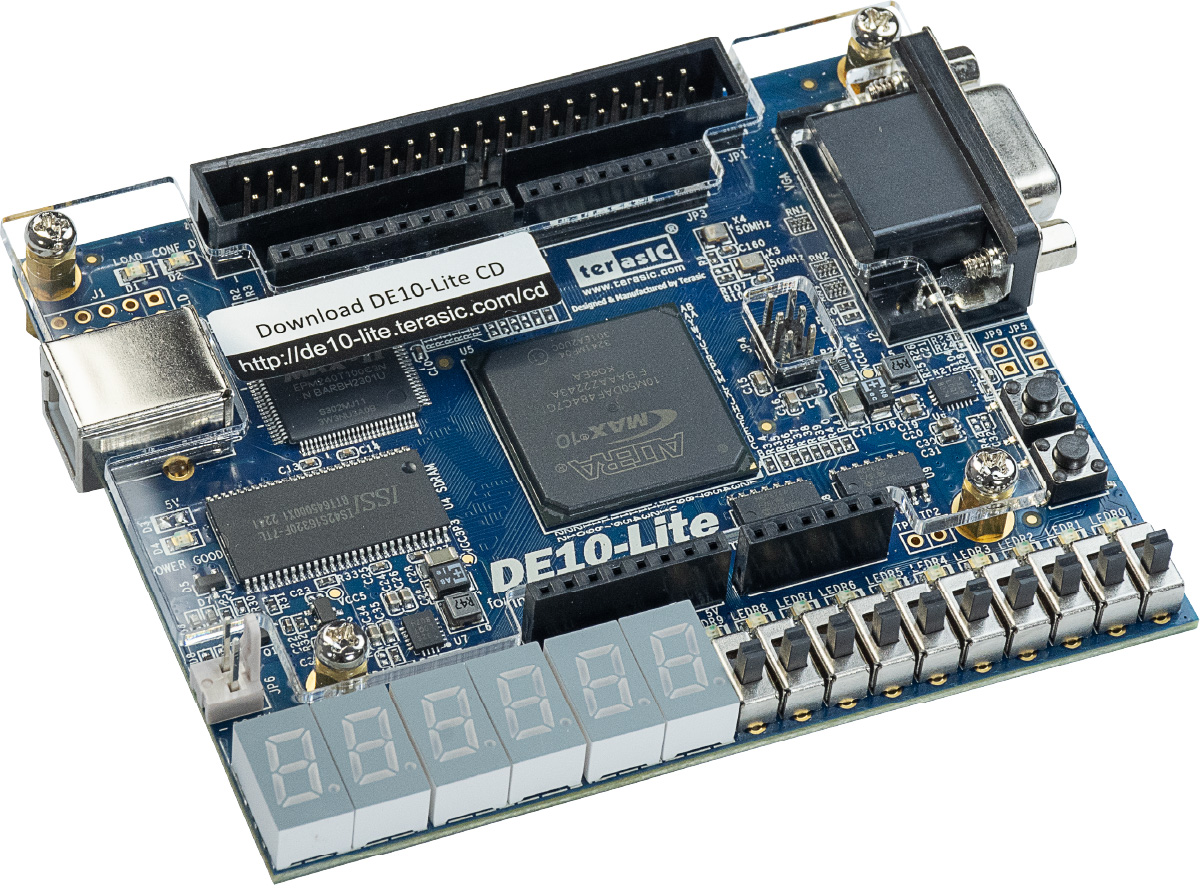
\includegraphics[width=0.5\linewidth]{img/DE10-Lite_45.jpg}
    \caption{DE10 lite dev. board}
    \label{fig:DE10-Lite_45}
\end{figure}

\newpage
\subsection{Overview of the LCD Display Used}

\begin{figure}[h!]
    \centering
    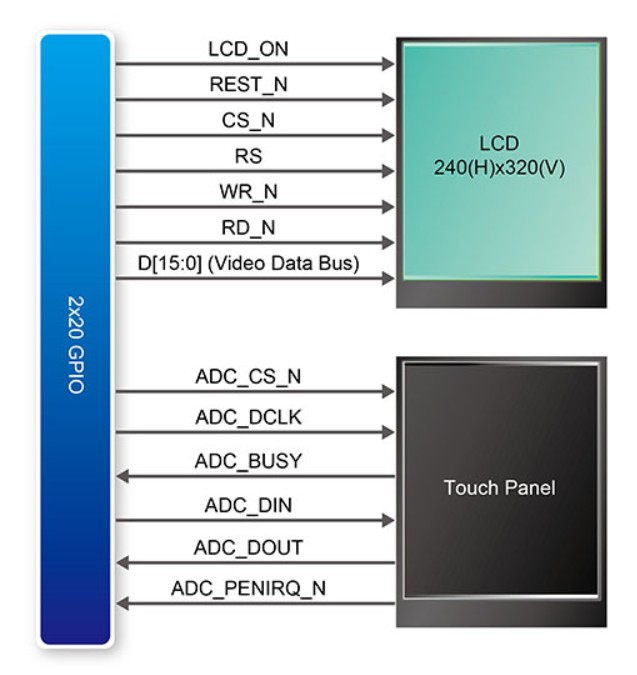
\includegraphics[width=0.5\linewidth]{img/LCD_block_diagram.jpg}
    \caption{LT24 LCD Display block diagram}
    \label{fig:LCD_block_diagram}
\end{figure}

\noindent
The LT24 LCD module integrates both a display panel and a resistive touch screen, which are interfaced using two different communication protocols. \
The touch panel uses an SPI interface to communicate with the AD7843 ADC integrated inside the module. \\
This device converts the analog touch coordinates into digital values, which are then read by the FPGA through the SPI bus. \\
The LCD panel is driven through a parallel bus interface, which is used to transmit pixel data for image rendering. \\
This interface allows the FPGA to directly write image data to the display for real-time visualization.

\newpage
\subsection{Fully connected Neural Network}

A fully connected neural network is a structure composed of basic elements called \textbf{neurons}, which are interconnected.

\vspace{1em}
\begin{figure}[h!]

    \begin{center}
        \resizebox{0.8\linewidth}{!}{
            \begin{tcolorbox}[neuralbox, width=0.95\linewidth]
            
                \centering
                
                \begin{neuralnetwork}[height=7.5]
                
                    \newcommand{\x}[2]{$x_#2$}
                    \newcommand{\y}[2]{$\hat{y}_#2$}
                    \newcommand{\hfirst}[2]{\small $h^{(1)}_#2$}
                    \newcommand{\hsecond}[2]{\small $h^{(2)}_#2$}
                
                    \inputlayer[count=3, bias=false, title=Input\\layer, text=\x]
                
                    \hiddenlayer[count=7, bias=false, title=Hidden\\layer 1, text=\hfirst]
                    \linklayers
                
                    \hiddenlayer[count=6, bias=false, title=Hidden\\layer 2, text=\hsecond]
                    \linklayers
                
                    \outputlayer[count=2, title=Output\\layer, text=\y]
                    \linklayers
                
                \end{neuralnetwork}
            
            \end{tcolorbox}
        }

    \end{center}

    \caption{Fully connected Deep Neural Network with two hidden layers}
    \label{fig:nn_architecture}

\end{figure}

\noindent
As shown in \autoref{fig:nn_architecture}, neurons are arranged in different layers; the output of the neurons in one layer becomes the input to the neurons in the next layer. \\
The first layer is called the \textbf{input layer}, and its inputs correspond to the inputs of the neural network to be processed. \\
The last layer is called the \textbf{output layer}, and its output represents the final processed output of the neural network. \\
The intermediate layers are called \textbf{hidden layers} and may not be present in some networks. \\
Networks with at least one hidden layer are referred to as deep neural networks.

\newpage
\subsubsection{Neuron structure}
To understand the behavior of a neural network, we must analyze the structure of a single neuron. 

\begin{figure}[h!]

    \begin{center}
    
        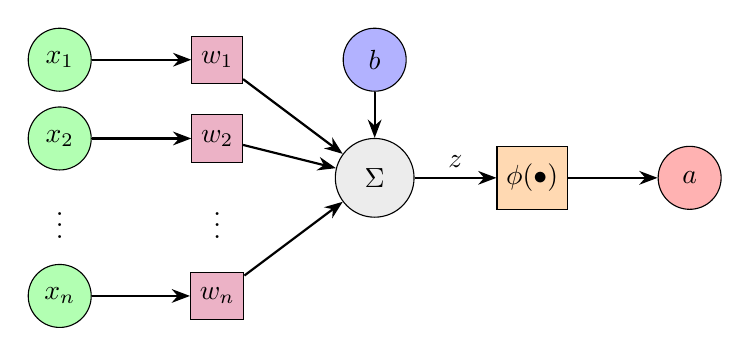
\begin{tikzpicture}[
            neuron/.style={circle, draw, minimum size=8mm, fill=green!30},
            weight/.style={rectangle, draw, minimum size=6mm, fill=purple!30},
            sum/.style={circle, draw, minimum size=10mm, fill=gray!15},
            act/.style={rectangle, draw, minimum size=8mm, fill=orange!30},
            output/.style={circle, draw, minimum size=8mm, fill=red!30},
            bias/.style={circle, draw, minimum size=8mm, fill=blue!30},
            arrow/.style={-{Stealth}, thick}
        ]
            
            % INPUTS
            \node[neuron] (x1) at (0,2) {$x_1$};
            \node[neuron] (x2) at (0,1) {$x_2$};
            \node (vdots) at (0,0) {$\vdots$};
            \node[neuron] (xn) at (0,-1) {$x_n$};
            
            % WEIGHTS
            \node[weight] (w1) at (2,2) {$w_1$};
            \node[weight] (w2) at (2,1) {$w_2$};
            \node (wdots) at (2,0) {$\vdots$};
            \node[weight] (wn) at (2,-1) {$w_n$};
            
            % SUM
            \node[sum] (s) at (4,0.5) {$\Sigma$};
        
            % OUTPUT
            \node[output] (a) at (8,0.5) {$a$};
        
            % BIAS
            \node[bias] (b) at (4,2) {$b$};
            
            % ACTIVATION FUNCTION
            \node[act] (phi) at (6,0.5) {$\phi(\bullet)$};
            
            % CONNECTIONS input -> weights
            \draw[arrow] (x1) -- (w1);
            \draw[arrow] (x2) -- (w2);
            \draw[arrow] (xn) -- (wn);
            
            % CONNECTIONS weights -> sum
            \draw[arrow] (w1) -- (s);
            \draw[arrow] (w2) -- (s);
            \draw[arrow] (wn) -- (s);
        
            % BIAS (from top)
            \draw[arrow] (b) -- (s);
            
            % SUM -> ACTIVATION (with z label)
            \draw[arrow] (s) -- (phi)
                node[midway, above] {$z$};
            
            % ACTIVATION -> OUTPUT
            \draw[arrow] (phi) -- (a);
        
        \end{tikzpicture}

    \end{center}

    \caption{Neuron block diagram structure}
    \label{fig:neuron_structure}

\end{figure}

\noindent
As we can see in \autoref{fig:neuron_structure}, a neuron is a basic computational unit that processes input data to produce an output following the \cref{eq:neuron_math_formula}

\begin{equation}
    \begin{cases}
        z_j &= \sum_i w_{ij} \cdot x_i + b_j \\
        a_j &= \phi(z_j)
    \end{cases}
    \label{eq:neuron_math_formula}
\end{equation}

\noindent
where:

\begin{itemize}
    \setlength\itemsep{0pt}
    \setlength\parskip{0pt}
    \item \(w_{ij}\): Weight of the j-th neuron associated to the i-th input
    \item \(x_i\): i-th input of the j-th neuron
    \item \(b_j\): bias of the j-th neuron
    \item \(z_j\): weighted sum of the j-th neuron
    \item \(\phi(\bullet)\): activation function of the j-th neuron
\end{itemize}

\noindent
The goal of using a neural network is to choose the correct values for the weights and biases of all neurons in order to obtain the desired output. \\
The process of choosing the weights and biases of the neurons is called the \textbf{Training process}. \\
The process of feeding inputs into the network to obtain its output is called the \textbf{Inference process}.

\newpage
\subsubsection{Inference Process}

For a neural network, the inference process consist on computing the output of every neuron and give them as input of the neuron of the next layer of the network. \\
To simplify the computation process the inputs and the outputs are stored in a vector and the weights are stored into matrix like is shown in \cref{eq:inf_matrix}.

\begin{equation}
    \begin{bmatrix}
        z_1 & \cdots & z_n
    \end{bmatrix}
    = 
    \begin{bmatrix}
        x_1 & \cdots & x_m
    \end{bmatrix} 
    \begin{bmatrix}
        w_{11} & \cdots & w_{1n} \\
        \vdots & \ddots & \vdots \\
        w_{m1} & \cdots & w_{mn}
    \end{bmatrix}
    +
    \begin{bmatrix}
        b_1 & \cdots & b_n
    \end{bmatrix}
    \label{eq:inf_matrix}
\end{equation}

\noindent
where:

\begin{itemize}
    \setlength\itemsep{0pt}
    \setlength\parskip{0pt}
    \item n: is the number of outputs of the network
    \item m: is the number of inputs of the network
\end{itemize}

\noindent
To obtain the output of a neuron layer, the weighted sum vector must pass through the activation function, like is shown in \cref{eq:act_funct}.

\begin{equation}
    \begin{bmatrix}
        a_1 & \cdots & a_n
    \end{bmatrix}
    = 
    \begin{bmatrix}
        \phi(z_1) & \cdots & \phi(z_n)
    \end{bmatrix}
    \label{eq:act_funct}
\end{equation}

\noindent
The activation functions can be various, but the most common ones are shown in \autoref{fig:activation_funct}

\begin{figure}[h!]
    \begin{center}
        \begin{tabular}{cc}
            
            % SIGMOID
            \begin{minipage}{0.45\textwidth}
                \centering
                \textbf{Sigmoid} $\sigma(x)$
                
                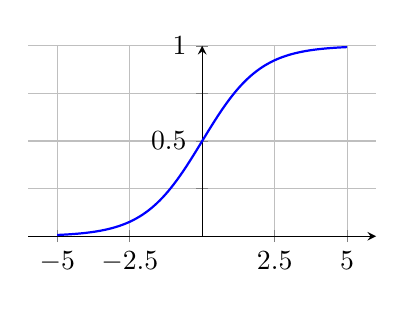
\begin{tikzpicture}
                    \begin{axis}[
                        width=6cm,
                        height=4cm,
                        axis lines=middle,
                        xmin=-6, xmax=6,
                        ymin=0, ymax=1,
                        xtick = {-5, -2.5, 0, 2.5, 5},
                        xticklabels = { $-5$, $-2.5$, $0$, $2.5$, $5$},
                        ytick = {0, 0.25, 0.5, 0.75, 1},
                        yticklabels = {$0$, , $0.5$, , $1$},
                        samples=100,
                        grid=both,
                    ]
                        \addplot[blue, thick] {1/(1+exp(-x))};
                    \end{axis}
                \end{tikzpicture}
            \end{minipage}
            
            &
            
            % TANH
            \begin{minipage}{0.45\textwidth}
                \centering
                \textbf{Tanh} $\tanh(x)$
                
                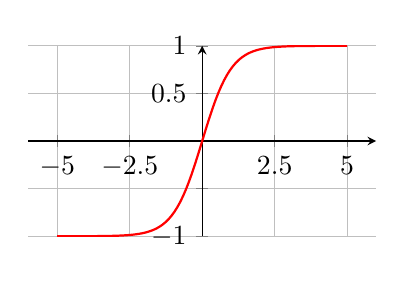
\begin{tikzpicture}
                    \begin{axis}[
                        width=6cm,
                        height=4cm,
                        axis lines=middle,
                        xmin=-6, xmax=6,
                        ymin=-1, ymax=1,
                        xtick = {-5, -2.5, 0, 2.5, 5},
                        xticklabels = { $-5$, $-2.5$, $0$, $2.5$, $5$},
                        ytick = {-1, -0.5, 0, 0.5, 1},
                        yticklabels = {$-1$, , $0$, $0.5$, $1$},
                        samples=100,
                        grid=both,
                    ]
                        \addplot[red, thick] {tanh(x)};
                    \end{axis}
                \end{tikzpicture}
            \end{minipage}
            
            \\[1em]
            
            % RELU
            \begin{minipage}{0.45\textwidth}
                \centering
                \textbf{ReLU}
                
                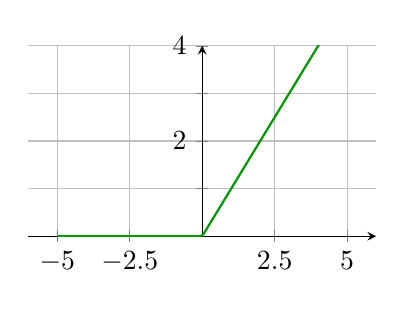
\begin{tikzpicture}
                    \begin{axis}[
                        width=6cm,
                        height=4cm,
                        axis lines=middle,
                        xmin=-6, xmax=6,
                        ymin=0, ymax=4,
                        xtick = {-5, -2.5, 0, 2.5, 5},
                        xticklabels = { $-5$, $-2.5$, $0$, $2.5$, $5$},
                        ytick = {0, 1, 2, 3, 4},
                        yticklabels = {$0$, , $2$, , $4$},
                        samples=100,
                        grid=both,
                    ]
                        \addplot[green!60!black, thick] {max(0,x)};
                    \end{axis}
                \end{tikzpicture}
            \end{minipage}
            
            &
            
            % LEAKY RELU
            \begin{minipage}{0.45\textwidth}
                \centering
                \textbf{Leaky ReLU}
                
                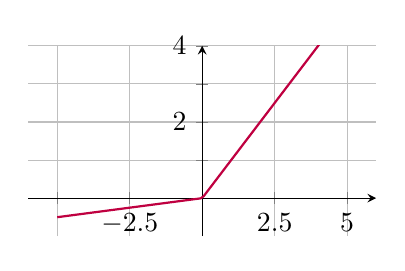
\begin{tikzpicture}
                    \begin{axis}[
                        width=6cm,
                        height=4cm,
                        axis lines=middle,
                        xmin=-6, xmax=6,
                        ymin=-1, ymax=4,
                        xtick = {-5, -2.5, 0, 2.5, 5},
                        xticklabels = { , $-2.5$, $0$, $2.5$, $5$},
                        ytick = {0, 1, 2, 3, 4},
                        yticklabels = {$0$, , $2$, , $4$},
                        samples=100,
                        grid=both,
                    ]
                        \addplot[purple, thick] {x > 0 ? x : 0.1*x};
                    \end{axis}
                \end{tikzpicture}
            \end{minipage}
            
        \end{tabular}
    \end{center}

    \caption{Most common activation functions}
    \label{fig:activation_funct}

\end{figure}

\subsubsection{Training Process}

During the training process, we need to send some inputs to the network and compare the obtained outputs with the desired ones. \\
Then, the weights and biases of the network must be modified to get closer to the desired output. \\
To train the network, an error function called the \textbf{cost function} is defined. This function represents the difference between the expected output of the network and the actual output, depending on the weights and biases of the network. \\
The goal of the training process is to choose the values of the weights and biases that minimize the cost function. \\
There are different types of cost functions, but the most common one is the quadratic cost function, defined in \cref{eq:quadratic_cost_funct}

\begin{equation}
    C(\vec{w},\vec{b}) = \frac{ || \vec{y} - \vec{a}_{\text{out layer}} || ^ 2 }{2}
    \label{eq:quadratic_cost_funct}
\end{equation}

\noindent
where:

\begin{itemize}
    \setlength\itemsep{0pt}
    \setlength\parskip{0pt}
    \item \(\vec{w}\): is the weight vector
    \item \(\vec{b}\): is the bias vector
    \item \(\vec{a}_{\text{out layer}}\): is the output vector
    \item \(\vec{y}\): is the desired output vector
\end{itemize}

\noindent
If we consider small changes in the weights and biases, we can approximate the variation of the cost function as

\[
    \Delta C \sim \vec{\nabla} C \cdot \Delta (\vec{w}, \vec{b})
\]

\noindent
where

\[
    \vec{\nabla} C = \left( \frac{\partial C}{\partial w_1}, \cdots, \frac{\partial C}{\partial w_{m \cdot n}}, \frac{\partial C}{\partial b_1}, \cdots, \frac{\partial C}{\partial b_n} \right)
\]

\noindent
We start with random values for the weights and biases of the network. \\
Then, each time we send an input to the network, we compute the gradient of the cost function and update the weights and biases to reduce the value of the cost function. \\
If we update the weight and bias vectors as shown in \cref{eq:update_weight_bias}

\begin{equation}
    \Delta (\vec{w}, \vec{b}) = - \eta \vec{\nabla} C
    \label{eq:update_weight_bias}
\end{equation}

\noindent
we obtain an always negative variation of the cost function (according to the approximation above) until we reach its minimum value. In fact,

\[
    \Delta C \sim \vec{\nabla} C \cdot \Delta (\vec{w}, \vec{b}) = - \eta 
    || \vec{\nabla} C || ^ 2 < 0 
\]

\noindent
There are various types of cost functions, but the important property is that every function used must have a minimum when \(\vec{y} = \vec{a}_{\text{out layer}}\). \\
It is easy to verify that the quadratic cost function satisfies this property, since it is a paraboloid.
    
    \newpage
    \section{Hardware implementation}
    
\subsection{NiosII CPU modules description}

The CPU hardware structure is made of different modules, and every module have his scope. \\
The main modules are:

\begin{itemize}
    \setlength\itemsep{0pt}
    \setlength\parskip{0pt}
    \item \textbf{Clock modules}: Used to manage the different clock sources.
    \item \textbf{Memory modules}: Used to connect the CPU to different memories, either internal or external to the chip.
    \item \textbf{Nios II modules}: Used to instantiate the CPU module and the system ID module.
    \item \textbf{PIO modules}: Used to instantiate the I/O peripherals. 
    \item \textbf{System peripherals}: Peripherals useful for programming and debugging, such as timers or UART devices.
    \item \textbf{LT24 modules}: Different modules used to control the LT24 LCD and touch screen (see \cite{rocketboards2024}). 
    \item \textbf{Floating-point operator module}: Used to instantiate hardware multipliers, dividers, and other floating-point operators.
\end{itemize}

\subsubsection{Clock Modules}

The clock section contains the modules required to generate and distribute the system clocks. \\
The \texttt{clk\_in} module provides the external reference clock, while the \texttt{system\_pll} module generates the internal clocks required by the system. \\
The \texttt{mm\_clock\_crossing\_bridge} module is used to connect components working on different clock domains.

\begin{figure}[h!]
    \centering
    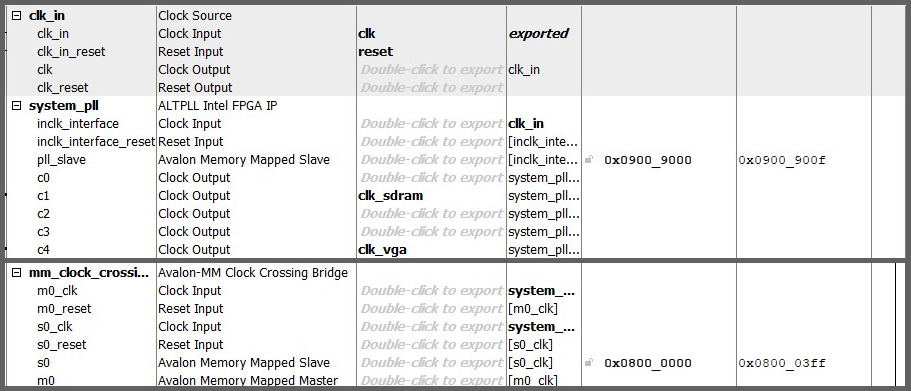
\includegraphics[width=1\linewidth]{img/clk_modules.jpg}
    \caption{CPU clock modules instantiated}
    \label{fig:clk_modules}
\end{figure}

\newpage

\subsubsection{Memory Modules}

The memory section contains the modules used for data and program storage. \\
The \texttt{onchip\_memory} module provides a small and fast internal memory, while the \texttt{sdram} module instantiate a controller for the external SDRAM memory to increase the available storage capacity.

\begin{figure}[h!]
    \centering
    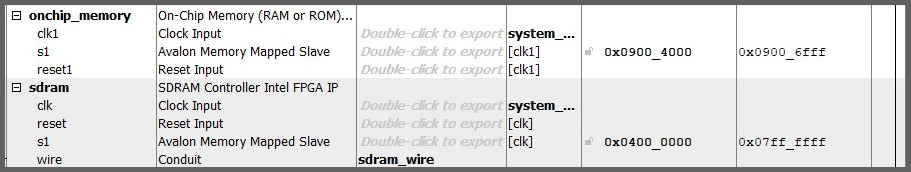
\includegraphics[width=1\linewidth]{img/memory_modules.jpg}
    \caption{CPU memory modules instantiated}
    \label{fig:memory_modules}
\end{figure}

\subsubsection{NiosII Modules}

The main processing section is based on the \texttt{nios2\_gen2} soft-core processor, which executes the software running on the FPGA. \\
The \texttt{sysid\_qsys} module is used to identify the generated system configuration and ensure software compatibility.

\begin{figure}[h!]
    \centering
    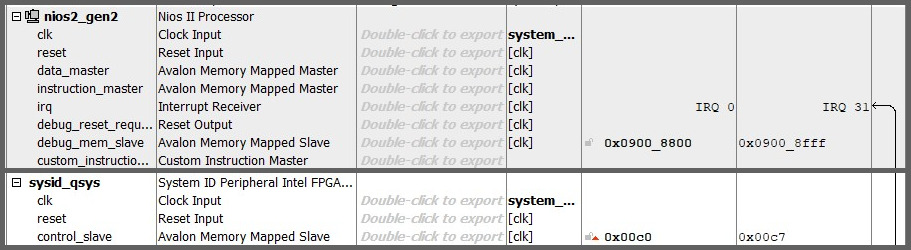
\includegraphics[width=1\linewidth]{img/nios2_modules.jpg}
    \caption{CPU (NiosII) modules instantiated}
    \label{fig:nios2_modules}
\end{figure}

\newpage

\subsubsection{PIO Modules}

The PIO modules are used to interface simple digital peripherals with the processor. \\
These modules manage input and output devices such as LEDs, switches, buttons, and other GPIO peripherals through memory-mapped registers.

\begin{figure}[h!]
    \centering
    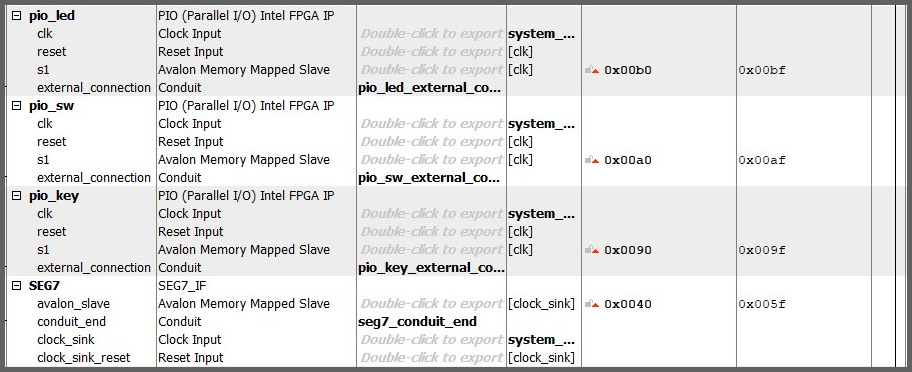
\includegraphics[width=1\linewidth]{img/pio_modules.jpg}
    \caption{CPU PIO modules instantiated}
    \label{fig:pio_modules}
\end{figure}

\subsubsection{System peripherals}

The system peripheral section contains modules used for communication and timing operations. \\
The \texttt{jtag\_uart} module allows serial communication and debugging through the JTAG interface, while the \texttt{timer} module provides timing and delay functionalities for the software running on the processor.

\begin{figure}[h!]
    \centering
    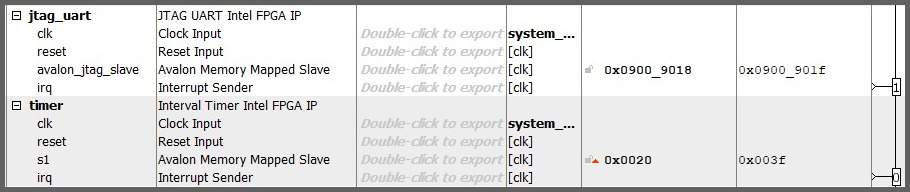
\includegraphics[width=1\linewidth]{img/system_perip_modules.jpg}
    \caption{CPU system peripherals instantiated}
    \label{fig:system_perip_modules}
\end{figure}

\newpage

\subsubsection{LT24 modules}

The LT24 section contains the modules required to control the LCD touchscreen display. \\
The \texttt{LT24\_Controller} module manages the communication with the display, while \texttt{LCD\_RESET\_N} handles the display reset signal. \\
The touchscreen interface is managed through the \texttt{touch\_panel\_spi}, \\\texttt{touch\_panel\_pen\_irq}, and \texttt{touch\_panel\_busy} modules.

\begin{figure}[h!]
    \centering
    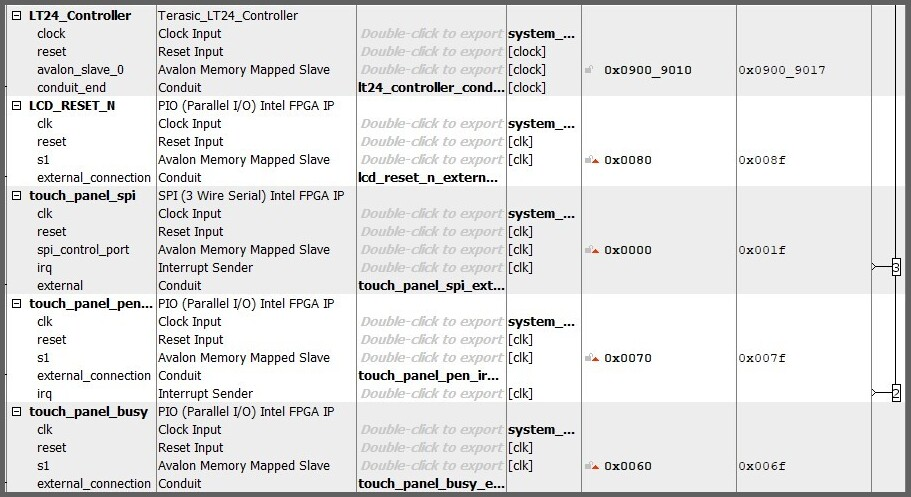
\includegraphics[width=1\linewidth]{img/LT24_modules.jpg}
    \caption{CPU LT24 modules instantiated}
    \label{fig:LT24_modules}
\end{figure}

\subsubsection{Floating-point operator module}

The floating-point operator module provides hardware support for floating-point arithmetic operations.

\begin{figure}[h!]
    \centering
    
\includegraphics[width=1\linewidth]{img/floating_point_module.jpg}
    \caption{CPU floating-point operator module instantiated}
    \label{fig:floating_point_module}
\end{figure}

\newpage
\subsection{Timing analysis}

This section defines the physical root clocks entering the device and characterizes the internal clock trees synthesized by the Phase-Locked Loop (PLL) hardware macro. \\
These constraints ensure that the Static Timing Analysis engine can accurately verify setup and hold timing margins across all clock domains.

\subsubsection{Timing configuration file}

The provided Synopsys Design Constraints (SDC) code snippet establishes the fundamental timing environment for the FPGA design.

\vspace{1em}
\begin{lstlisting}[language=sdc, caption=Base clock settings for timing analyzer, label={lst:base_clock_settings}]
    create_clock    
        -name {altera_reserved_tck} 
        -period 100.000 
        -waveform { 0.000 50.000 } 
        [get_ports {altera_reserved_tck}]
    create_clock 
        -name {ADC_CLK_10} 
        -period 100.000 
        -waveform { 0.000 50.000 } 
        [get_ports {ADC_CLK_10}]
    create_clock    
        -name {MAX10_CLK1_50} 
        -period 20.000 
        -waveform { 0.000 10.000 } 
        [get_ports {MAX10_CLK1_50}]
                    
    derive_pll_clocks
\end{lstlisting}

\noindent
The base clocks settings present in \autoref{lst:base_clock_settings} represent physical, periodic signals routed from external oscillators on the board to specific input ports of the FPGA.

\begin{itemize}
    \item \texttt{altera\_reserved\_tck} \\
    is dedicated to the asynchronous JTAG Test Clock tap for hardware debugging. 

    \item \texttt{ADC\_CLK\_10} \\
    is the \(10\ \text{MHz}\) clock used to drive the controller of the LT24 touchscreen.
    
    \item \texttt{MAX10\_CLK1\_50} \\
    these serve as the primary external reference clocks feeding the internal logic and PLL inputs.

    \item \texttt{derive\_pll\_clocks} \\
    this command instructs Intel Quartus Prime to automatically detect internal PLL instances.

\end{itemize}

\noindent
Generated clocks represent signals derived from an existing master clock inside the FPGA, altered via frequency multiplication, division, or phase shifts.

\vspace{1em}
\begin{lstlisting}[language=sdc, caption=Generated clock settings for timing analyzer]
    create_generated_clock 
        -name {clk_dram_ext} 
        -source [get_pins{ u0|system_pll|sd1|pll7|clk[1] }] 
        [get_ports {DRAM_CLK}] 
    create_generated_clock  
        -name {u0|system_pll|sd1|pll7|clk[0]} 
        -source [get_pins{u0|system_pll|sd1|pll7|inclk[0]}] 
        -duty_cycle 50/1 -multiply_by 2 
        -master_clock {MAX10_CLK1_50} 
        [get_pins {u0|system_pll|sd1|pll7|clk[0]}] 
    create_generated_clock  
        -name {u0|system_pll|sd1|pll7|clk[3]} 
        -source [get_pins{u0|system_pll|sd1|pll7|inclk[0]}] 
        -duty_cycle 50/1 -multiply_by 1 
        -divide_by 5 -master_clock {MAX10_CLK1_50} 
        [get_pins{u0|system_pll|sd1|pll7|clk[3]}] 
\end{lstlisting}

\noindent
The paths originating from the switches and push-buttons were subsequently defined as asynchronous (unconstrained), while timing constraints were also specified for the paths driving the seven-segment displays and leds.

\vspace{1em}
\begin{lstlisting}[language=sdc, caption=Paths constraints for asynchronous buttons and leds on the board]
    set_false_path 
        -from [get_ports {SW[*] KEY[*]}] 
    set_false_path 
        -from [get_ports {LT24_ADC_*}] 
    set_false_path 
        -to [get_ports {HEX0[*] HEX1[*] HEX2[*] HEX3[*]
                        HEX4[*] HEX5[*] LEDR[*]}]
\end{lstlisting}

\noindent
Furthermore, based on the timing specifications provided in the corresponding datasheets, minimum and maximum output delays were defined for both the SDRAM interface and the JTAG Debug Module (USB Blaster). \\
The timing constraints for the JTAG Debug Module (USB Blaster) were derived using the forum \cite{altera_jtag_constraints_2026}. \\
For the LT24 display interface, since it is not directly synchronized to the system clock and all timing requirements are handled internally by a controller operating at \(10 \; \text{MHz}\), arbitrary minimum and maximum output delay values (\(1 \; \text{ns}\) in this implementation) were assigned relative to the clock signal. \\
In this case, verifying synchronization with the clock is sufficient to guarantee correct timing behavior, as the LT24 controller itself enforces the required interface timing.

\vspace{1em}
\begin{lstlisting}[language=sdc, caption=Paths constraints for SDRAM]
    set_input_delay 
        -add_delay -max -clock [get_clocks {clk_dram_ext}]  
        5.900 [get_ports {DRAM_DQ[*]}]
    set_input_delay 
        -add_delay -min -clock [get_clocks {clk_dram_ext}]  
        3.000 [get_ports {DRAM_DQ[*]}]
    set_output_delay 
        -add_delay -max -clock [get_clocks {clk_dram_ext}]
        1.600 [get_ports {DRAM_ADDR[*]}]
    set_output_delay 
        -add_delay -min -clock [get_clocks {clk_dram_ext}]  
        -0.900 [get_ports {DRAM_ADDR[*]}]
\end{lstlisting}

\begin{lstlisting}[language=sdc, caption=Paths constraints for LT24 module]
    set_output_delay 
        -add_delay  
        -clock [get_clocks {u0|system_pll|sd1|pll7|clk[3]}]  
        1.000 [get_ports {LT24_*}]
\end{lstlisting}

\begin{lstlisting}[language=sdc, caption=Paths constraints for JTAG Debug Module (USB Blaster)]
    set_input_delay 
        -add_delay -max 
        -clock [get_clocks {altera_reserved_tck}]  
        10.000 [get_ports {altera_reserved_tdi}]
    set_input_delay 
        -add_delay -min 
        -clock [get_clocks {altera_reserved_tck}]  
        2.000 [get_ports {altera_reserved_tdi}]
    set_input_delay 
        -add_delay -max 
        -clock [get_clocks {altera_reserved_tck}]  
        10.000 [get_ports {altera_reserved_tms}]
    set_input_delay 
        -add_delay -min 
        -clock [get_clocks {altera_reserved_tck}]  
        2.000 [get_ports {altera_reserved_tms}]
    set_output_delay 
        -add_delay -max 
        -clock [get_clocks {altera_reserved_tck}]  
        10.000 [get_ports {altera_reserved_tdo}]
    set_output_delay 
        -add_delay -min 
        -clock [get_clocks {altera_reserved_tck}]  
        2.000 [get_ports {altera_reserved_tdo}]  
\end{lstlisting}

\newpage
\subsubsection{Maximum Frequency Report}
The timing analyzer uses the library of the FPGA macro-cells to verify that the timing constraints are respected for both the slow and fast models.\\
The slow model is used to check the maximum frequency of the clock sources (at a temperature of \(85^\circ C\) worst case) and the setup timing constraints.\\
The fast model is used to verify that hold time violations do not occur (at a temperature of \(0^\circ C\) best case).

\begin{figure}[h!]
    \centering
    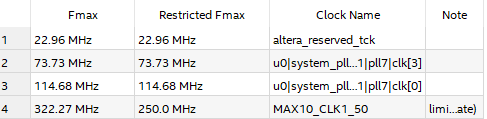
\includegraphics[width=\textwidth]{img/timing_analyzer_fmax.png}
    \caption{Maximum frequency Timing analyzer report}
    \label{fig:timing_analyzer_fmax}
\end{figure}

\begin{itemize}
    \item \texttt{Internal System Clock (clk[0])} \\
    The Nios II CPU and all associated modules meet the timing requirements. Since the maximum achievable frequency ($114.68 \; \text{MHz}$) exceeds the target frequency ($100 \; \text{MHz}$), the system operates with positive timing slack.

    \item \texttt{LT24 Display Clock (clk[3])} \\
    Although the internal logic could theoretically operate up to $73.73 \; \text{MHz}$, only $10 \; \text{MHz}$ is required for the LT24 interface. As specified in the LT24 datasheet, higher frequencies may cause data corruption; therefore, the clock frequency is kept at or below $10 \; \text{MHz}$ despite the available timing margin.

    \item \texttt{JTAG Debug Clock (altera\_reserved\_tck)} \\
    The timing analysis confirms compliance with the required $10 \; \text{MHz}$ operating frequency.
\end{itemize}

\noindent
\textit{Note: The timing analyzer indicates that while the internal silicon routing from this clock pin is capable of supporting frequencies up to $322.27 \; \text{MHz}$, the physical I/O buffer architecture of the MAX 10 device imposes a hard limit at $250.0 \; \text{MHz}$. \\
This limitation is due to the electrical switching capability of the I/O transistors, which cannot reliably toggle beyond this frequency. \\
However, this constraint is not a concern in practice, since the operating frequency of $50 \; \text{MHz}$ is well below both the I/O limit ($250 \; \text{MHz}$) and the internal routing limit ($322.27 \; \text{MHz}$), resulting in a substantial safety margin for this clock domain. Quartus therefore caps the reported maximum frequency at $250 \; \text{MHz}$ to prevent unrealistic external clock assumptions in future design iterations.}

\newpage

\subsubsection{Hold and Setup Time Slack Report}
The timing analyzer evaluates the setup and hold slack for each clock domain to ensure correct data latching and prevent metastability. \\
The setup analysis checks that the data arrives at the destination register before the next clock edge, whereas the hold analysis ensures the data remains stable long enough after the clock edge to be properly sampled. \\
As shown in the \autoref{fig:timing_slack_reports}, all clock domains exhibit positive slack, confirming that the design fully meets all timing requirements under both worst-case and best-case operating conditions.

\begin{figure}[h!]
    \centering
    \begin{subfigure}[b]{0.48\textwidth}
        \centering
        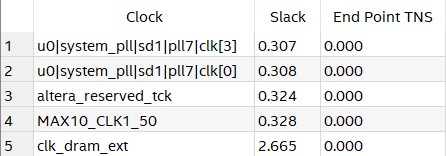
\includegraphics[width=\textwidth]{img/hold_summary.jpg}
        \caption{Hold summary report}
        \label{fig:hold_summary}
    \end{subfigure}
    \hfill
    \begin{subfigure}[b]{0.48\textwidth}
        \centering
        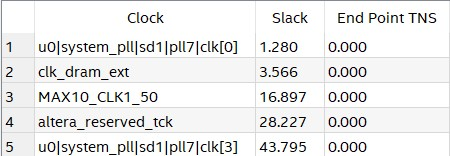
\includegraphics[width=\textwidth]{img/setup_summary.jpg}
        \caption{Setup summary report}
        \label{fig:setup_summary}
    \end{subfigure}
    \caption{Hold and Setup slack Timing analyzer reports}
    \label{fig:timing_slack_reports}
\end{figure}

\begin{itemize}
    \item \texttt{Internal System Clock (clk[0])} \\
    The system clock meets both timing constraints comfortably. It presents a worst-case hold slack of $0.308 \; \text{ns}$ and a setup slack of $1.280 \; \text{ns}$. The positive margins ensure stable synchronous operations within the Nios II CPU and its peripherals.

    \item \texttt{LT24 Display Clock (clk[3])} \\
    The clock domain dedicated to the LT24 display interface reports a hold slack of $0.307 \; \text{ns}$ and a substantial setup slack of $43.795 \; \text{ns}$. This significant setup margin is a direct consequence of the relaxed operating frequency ($10 \; \text{MHz}$) compared to the maximum frequency supported by the internal logic routing.

    \item \texttt{External DRAM Clock (clk\_dram\_ext)} \\
    The external memory clock domain exhibits high robust timing margins, showing a hold slack of $2.665 \; \text{ns}$ and a setup slack of $3.566 \; \text{ns}$. This ensures reliable data transfer with the external SDRAM chip.

    \item \texttt{System Input Clock (MAX10\_CLK1\_50)} \\
    The $50 \; \text{MHz}$ main input clock shows a hold slack of $0.328 \; \text{ns}$ and a setup slack of $16.897 \; \text{ns}$, confirming safe propagation of the external reference clock into the internal PLL structures.

    \item \texttt{JTAG Debug Clock (altera\_reserved\_tck)} \\
    The JTAG test clock complies with the constraints, reporting a hold slack of $0.324 \; \text{ns}$ and a setup margin of $28.227 \; \text{ns}$.
\end{itemize}

\newpage
\subsection{Resource Usage}
\label{sssec:hw_footprint_chpl}

Compared to all the resources available on the chip, the total logic elements used are only \(17\%\) of the total, and the total memory bits used are \(11\%\), as shown in \autoref{fig:resorces_usage}. \\
Furthermore only 16 of the 288 embedded multipliers and one of the four internal PLL.

\begin{figure}[h!]
    \centering
    \begin{subfigure}[t]{0.45\textwidth}
        \centering
        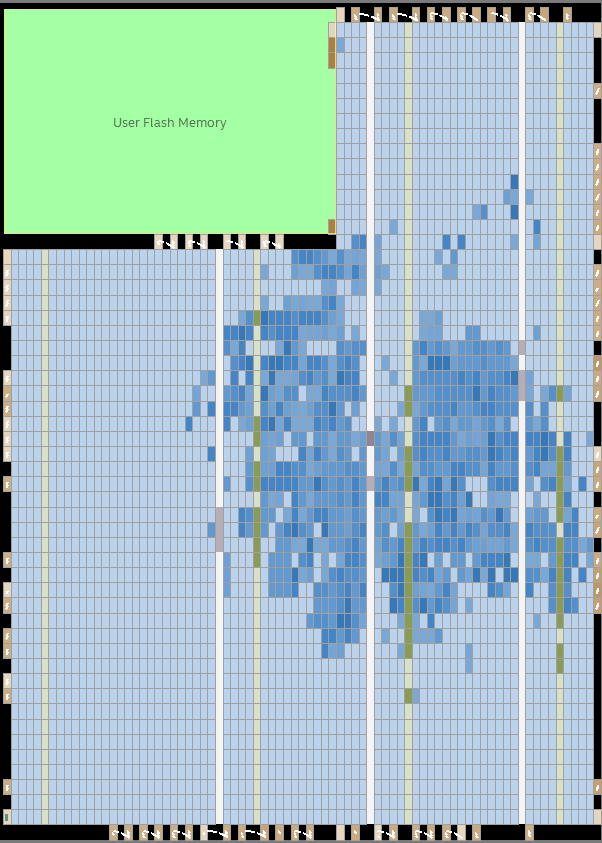
\includegraphics[width=\textwidth]{img/chip_planner_view.png} 
        \caption{Hardware-Footprint on Chip Planner}
        \label{fig:chip_planner_view}
    \end{subfigure}
    \hfill 
    \begin{subfigure}[t]{0.45\textwidth}
        \centering
        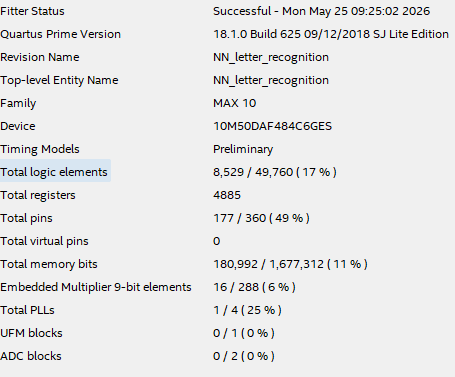
\includegraphics[width=\textwidth]{img/fitter_summary.png} 
        \caption{Fitter summary hardware used}
        \label{fig:fitter_summary}
    \end{subfigure}
    
    \caption{FPGA resources usage}
    \label{fig:resorces_usage}
\end{figure}

        
    \newpage
    \section{Software implementation}
    The software architecture is divided into two main parts. \\
\textbf{Neural Network implementation} is based on two different libraries:

\begin{itemize}

    \setlength\itemsep{0pt}
    \setlength\parskip{0pt}
    
    \item \textbf{Matrix Library}: responsible for matrix operations and mathematical computations required by the neural network.
    
    \item \textbf{Neural Network Library}: handles the initialization and execution of a fully connected neural network composed of three layers.
\end{itemize}

\noindent
\textbf{Graphical User Interface (GUI) implementation} relies on two dedicated libraries used to manage communication with the display and the touchscreen:

\begin{itemize}

    \setlength\itemsep{0pt}
    \setlength\parskip{0pt}
    
    \item \textbf{LCD Display Control Library}: handles everything related to displaying images on the LCD screen.
    
    \item \textbf{SPI-Based Touchscreen Control Library}: manages communication with the touchscreen using the Serial Peripheral Interface (SPI).
\end{itemize}

\subsection{Neural Network implementation}

The Neural Network library folder tree is shown in \autoref{fig:NN_folder_tree}

\begin{figure}[h!]
    \begin{center}
        \scalebox{0.85}{
            \begin{tikzpicture}%
               \draw[color=black!60!white]
                \FTdir(\FTroot,root,NN\_letter\_recognition){
                
                ++(0,-0.5em)
                
                \FTdir(root,LUT,LUT){
                    \FTdir(LUT,functions,functions){
                        \FTfileC(functions,activation\_functions.c)
                        \FTfileC(functions,functions.c)
                        \FTfileH(functions,functions.h)   
                    }
                    \FTdir(LUT,weight-and-bias,weight\_and\_bias){
                        \FTfileH(weight-and-bias,weight\_and\_bias.h)
                        \FTfileC(weight-and-bias,weight\_matrix\_emnist.c)
                        \FTfileC(weight-and-bias,weight\_matrix\_mnist.c)
                    }

                    ++(0,-0.5em)
    
                    \FTdir(LUT,m1,...)
                }

                ++(0,-0.5em)

                \FTdir(root,NN-lib,NN\_lib){
                    \FTfileC(NN-lib,matrix\_lib.c)
                    \FTfileH(NN-lib,matrix\_lib.h)   
                    \FTfileH(NN-lib,NN\_lib\_debug.h)   
                    \FTfileC(NN-lib,NN\_lib.c)
                    \FTfileH(NN-lib,NN\_lib.h)  
                }

                ++(0,-0.5em)

                \FTdir(root,m2,...)

            };

            \end{tikzpicture}
        }
    \end{center}

    \caption{Neural Network library function folder tree}
    \label{fig:NN_folder_tree}
    
\end{figure}

\noindent
To implement the neural network, a matrix library has been created to define all the operations that have to be performed with matrices, and a neural network library has been created to define the network and connect all the layers together.

\newpage
\subsubsection{Matrix Library}
\label{sssec:matrix_library}

This library contains the \texttt{Matrix} type, which is a structure defined in \autoref{lst:Matrix_typedef}.

\vspace{1em}
\begin{lstlisting}[language=C, caption={Matrix type}, label={lst:Matrix_typedef}, morekeywords={Matrix}]
    typedef struct{
        unsigned int row;
        unsigned int col;
        float *data;
    }Matrix;
\end{lstlisting}

\noindent
The \texttt{Matrix} type contains the fields \texttt{row} and \texttt{col}, which store the number of rows and columns of the matrix, and the field \texttt{*data}, which is a pointer to the matrix data. \\
This type is defined to represent a matrix of floating-point values only, since the weights of the neural network are of type \texttt{float}. \\
To create a matrix variable, the \texttt{malloc()} function must be used to allocate memory in the heap. \\
In \texttt{matrix\_lib.h}, several functions are defined to instantiate a matrix variable (constructors) and to release its memory (destructor) shown in \autoref{lst:Matr_constr_destr}.

\vspace{1em}
\begin{lstlisting}[language=C, caption={Constructors and Destructor}, label={lst:Matr_constr_destr}, morekeywords={Matrix}]
    /* ---------------- Constructors ------------------ */
    static inline Matrix matrix_error(void) {
        return (Matrix){0, 0, NULL};
    }
    
    Matrix matrix_init(unsigned int row, unsigned int col);
    ...             
    Matrix matrix_null(unsigned int row, unsigned int col);

    /* ----------------- Destructors ------------------- */
    void matrix_free(Matrix *m);
\end{lstlisting}

\newpage
\noindent
To instantiate a matrix variable the syntax is shown in \autoref{lst:matrix_usage}.

\vspace{1em}
\begin{lstlisting}[language=C, caption={Matrix usage example}, label={lst:matrix_usage}, morekeywords={Matrix}]
    int main(void){
        Matrix m = matrix_init(ROW_NUM, COL_NUM);

        Matrix error_m = matrix_error();
        if(matrix_compare(&error_m, &m) == 1){
            printf("ERROR: Matrix initialization failure");
            return 0;   // Exit failure
        }
        
        ...
        
        matrix_free(&m);
        return 1;   // Exit success
    }
\end{lstlisting}

\noindent
The \texttt{matrix\_error(void)} constructor is used only to return an empty Matrix, useful to identify an error in a \texttt{Matrix} return type function as shown in \autoref{lst:matrix_usage}. \\
Since \texttt{matrix\_error(void)} don't allocate data into dynamic memory (is an empty matrix) the destructor must not be used. \\
In this library, the most common matrix operations such as addition, multiplication, transposition, etc., have also been defined.\\
Most of the operations are implemented as functions that return an integer value representing the status; if the return value is 1, the operation has been completed successfully; otherwise, the operation has encountered a problem and cannot be executed correctly.

\newpage
\subsubsection{Neural Network Library}

This library contains the \texttt{NN\_f\_conn} type, which is a structure defined in 
\autoref{lst:NN_typedef}

\vspace{1em}
\begin{lstlisting}[language=C, caption={NN\_f\_conn type}, label={lst:NN_typedef}, morekeywords={NN\_f\_conn, Matrix}, alsoletter={\_}]
    typedef struct{
        
        Matrix w1;
        Matrix b1;
    
        Matrix w2;
        Matrix b2;
    
        Matrix w3;
        Matrix b3;
    
    }NN_f_conn;
\end{lstlisting}

\noindent
With this structure can be defined fully connected neural network with three layers:

\begin{itemize}
    \setlength\itemsep{0pt}
    \setlength\parskip{0pt}
    \item The input layer
    \item An hidden layer
    \item The output layer
\end{itemize}

\noindent
This structure contains three pairs of matrices defined with the \texttt{Matrix} type described in \autoref{sssec:matrix_library}. \\
Each pair of matrices represents the weights and biases of a layer of the fully connected neural network. \\
The neural network is initialized using the function \texttt{NN\_init()}, which initializes all the matrices with the correct dimensions. \\
Since the matrices contain data arrays allocated using the \texttt{malloc()} function, the \texttt{free()} function must be used to de-allocate them; the function that de-allocates all the network data is \texttt{NN\_free()} as shown in \autoref{lst:NN_constr_destr}.

\vspace{1em}
\begin{lstlisting}[language=C, caption={Constructors and Destructor}, label={lst:NN_constr_destr}, morekeywords={NN\_f\_conn, Matrix}, alsoletter={\_}]
    /* ---------------- Constructors ------------------ */
    NN_f_conn NN_init(void);

    /* ----------------- Destructors ------------------- */
    void NN_free(NN_f_conn *nn);
\end{lstlisting}

\noindent
The dimensions of the network layers are defined in another file located in the \texttt{./LUT/weight\_and\_bias} directory, named \texttt{weight\_and\_bias.h}. \\
In this file, a global \texttt{Matrix} vector is defined, which contains all the weights and biases of the network. \\
To identify at which index each matrix is stored, a global enumeration variable has been defined, as shown in \autoref{lst:NN_enum_index}.

\vspace{1em}
\begin{lstlisting}[language=C, caption={Enumerate variable to identify the NN index}, label={lst:NN_enum_index}, morekeywords={NN\_weight\_index}, alsoletter={\_}]
    typedef enum{
        
        WEIGHT_NN_1 = 0,
        BIAS_NN_1 = 3,
    
        WEIGHT_NN_2 = 1,
        BIAS_NN_2 = 4,
    
        WEIGHT_NN_3 = 2,
        BIAS_NN_3 = 5,
    
    }NN_weight_index;
\end{lstlisting}

\noindent
Since the network used for the MNIST dataset and the EMNIST dataset is, in both cases, a three-layer fully connected network (with a different number of neurons in each layer), conditional compilation is used in the header file to load one network or the other, as shown in \autoref{lst:NN_weight_sel}.

\vspace{1em}
\begin{lstlisting}[language=C, caption={NN selection with conditional compilation}, label={lst:NN_weight_sel}, morekeywords={Matrix,\#include,\#define,\#ifdef,\#ifndef,\#else,\#endif}, alsoletter={\#}]
    // Comment this line to use the EMNIST dataset
    // (letters and numbers) instead of MNIST (only numbers)
    #define MNIST_DATASET

    #ifdef MNIST_DATASET
        #define WEIGHT_AND_BIAS weight_and_bias_mnist
        extern Matrix weight_and_bias_mnist[6];
    #else
        #define WEIGHT_AND_BIAS weight_and_bias_emnist
        extern Matrix weight_and_bias_emnist[6];
    #endif
\end{lstlisting}

\noindent
\texttt{weight\_and\_bias\_mnist[6]} and \texttt{weight\_and\_bias\_emnist[6]} are two constant arrays of type \texttt{Matrix}, defined respectively in \\
\texttt{./LUT/weight\_and\_bias/weight\_and\_bias\_mnist.c} and \\
\texttt{./LUT/weight\_and\_bias/weight\_and\_bias\_emnist.c}.

\noindent
These matrix vectors contain the weights and biases for the MNIST and EMNIST networks. 

\newpage
\noindent
Inside \texttt{NN\_lib}, the \texttt{NN\_init()} function uses the \texttt{WEIGHT\_AND\_BIAS} define to access the constant matrices associated with the correct dataset. \\
The operation that can be performed are shown in \autoref{lst:NN_operations}

\vspace{1em}
\begin{lstlisting}[language=C, caption={NN\_lib functions defined}, label={lst:NN_operations}, morekeywords={Matrix,\#include,\#define,\#ifdef,\#ifndef,\#else,\#endif}, alsoletter={\#}]
    /* ---------------- Operations -------------------- */
    int forw_prop(Matrix input, 
                  Matrix *out, 
                  NN_f_conn *nn, 
                  void (*activation_funct)(Matrix *a));
    char nn_output_convert(Matrix input);
    
    /* ------------- Activation functions ------------- */
    void relu_funct(Matrix *a);
    void leaky_relu_funct(Matrix *a);
    void tanh_funct(Matrix *a);
    void sigmoid_funct(Matrix *a);
\end{lstlisting}

\noindent
The \texttt{forw\_prop()} function takes a \texttt{Matrix} type input and produces a \texttt{Matrix} output from the \texttt{NN\_f\_conn} neural network, using activation functions passed as function pointers. \\
Several activation functions are defined; the most computationally expensive ones are implemented using look-up tables stored in \\
\texttt{./LUT/functions/functions.h}. \\
The function \texttt{nn\_output\_convert} determines which neural network has been selected and returns the corresponding output character from the input matrix, where the input matrix is the result computed by the network.

\newpage
\subsection{GUI implementation}
The GUI library folder tree is shown in \autoref{fig:GUI_lib_folder_tree}

\begin{figure}[h!]
    \begin{center}
        \scalebox{0.85}{
            \begin{tikzpicture}%
               \draw[color=black!60!white]
                \FTdir(\FTroot,root,NN\_letter\_recognition){
    
                    ++(0,-0.5em)
                    
                    \FTdir(root,graphic-matrix-lib,graphic\_matrix\_lib) {
                        \FTfileH(graphic-matrix-lib,debug\_graphic\_lib.h)
                        \FTfileC(graphic-matrix-lib,simple\_graphics\_matrix.c)
                        \FTfileH(graphic-matrix-lib,simple\_graphics\_matrix.h)
                    }
                    
                    %++(0,-0.5em)
    
                    \FTdir(root,gui,gui) {
                        \FTfileH(gui,gui\_config.h)
                        \FTfileH(gui,gui\_debug.h)
                        \FTfileC(gui,gui.c)
                        \FTfileH(gui,gui.h)
                    }

                    ++(0,-0.5em)

                    \FTdir(root,...,...){}
    
                };

            \end{tikzpicture}
        }
    \end{center}

    \caption{GUI library function folder tree}
    \label{fig:GUI_lib_folder_tree}
    
\end{figure}

\noindent
The GUI library handles the operations needed to render the user interface on the display and enables touchscreen sensitivity, allowing the user to handwrite their desired character.

\vspace{1em}
\begin{lstlisting}[language=C, caption={GUI initialization}, label={lst:GUI_init}]
    void GUI_init(alt_video_display *pDisplay, 
                  DESK_INFO *DeskInfo, 
                  RECT *rcTouch)
    {
        // Init LCD
        LCD_Init();
        
        // Clean LCD
        vid_clean_screen(pDisplay, BACKGROUND_COLOR);
        
        // Wait 1s
        usleep(1*1000*1000);
        
        (*DeskInfo).Button_Index = PEN_BUTTON;
        
        GUI_DeskInit(pDisplay, DeskInfo);
        GUI_DeskDraw(pDisplay, DeskInfo);
        GUI_SymbolsDraw(pDisplay, DeskInfo, 0);
        
        RectCopy(rcTouch, &(*DeskInfo).rcPaint);
        RectInflate(rcTouch, -2-DOT_SIZE, -2-DOT_SIZE);
    }
\end{lstlisting}

\newpage
\noindent
During initialization, the program builds and displays the interface \\ (\texttt{GUI\_init()}), through functions like \texttt{GUI\_DeskInit()}, \texttt{GUI\_DeskDraw()}, \\
\texttt{GUI\_SymbolsDraw()}. \\
Then (\autoref{lst:Touch_screen_GetXY}) it then enters a while loop that continuously detects (an alarm is implemented) the pointer's position \texttt{Touch\_GetXY()}, based on where the pen presses down. The task of checking whether the pointer is inside a specific section of the display is handled by the library function  \texttt{IsPtInRect()}. 

\vspace{1em}
\begin{lstlisting}[language=C, caption={Handling the touchscreen}, label={lst:Touch_screen_GetXY}]
    if(Touch_GetXY(pTouch, &X, &Y)){
    
        PtSet(&Pt, X, Y);
        int ButtonId = GUI_CheckButton(DeskInfo, &Pt);
    
        GUI_DEBUG_TOUCH_PRINTF("x=%d, y=%d\r\n", X, Y);
        GUI_DEBUG_TOUCH_PRINTF("Button index=%d\n", 
                               (*DeskInfo).Button_Index);
    
        if (IsPtInRect(&Pt, rcTouch) &&  
            (*DeskInfo).Button_Index == PEN_BUTTON){
            // Touch inside drawing area
            if (Pt_prev.x != -1 && Pt_prev.y != -1)
                vid_draw_sloped_line_on_matrix( Pt_prev.x,
                Pt_prev.y, Pt.x, Pt.y, DOT_SIZE, BLACK_24,
                pDisplay, &drawing_grayscale_m);
            else
                vid_draw_circle_on_matrix(Pt.x, Pt.y,
                DOT_SIZE, BLACK_24, DO_FILL, pDisplay,
                &drawing_grayscale_m);
    
            PtSet(&Pt_prev, X, Y);    
        }
    }
\end{lstlisting}

\noindent
To draw the pen strokes, we used the\\
\texttt{vid\_draw\_sloped\_line\_on\_matrix()} function. \\
This "interpolates" the detected touchpoints by connecting them with a sloped line. \\
This approach gives us a very smooth drawing and writing experience without needing to bump up the touch-detection refresh rate, avoiding extra overhead.

\newpage
\noindent
On the other hand, if a press is detected on one of the available virtual buttons (or icons), the system behaves differently:

\begin{itemize}

    \setlength\itemsep{0pt}
    \setlength\parskip{0pt}
    
    \item \texttt{BACKSPACE\_BUTTON}: deletes the last character written in the letter box at the top of the display. If the letter box fills up, the last entered character is overwritten.
    
    \item \texttt{PEN\_BUTTON}: enables pen writing exclusively within the dedicated drawing area. There is a timer that triggers once the pen is lifted; when it times out, the data saved in the 140x140 matrix is downscaled to a 28x28 grayscale matrix, by the \texttt{downscale\_matrix()} function, and fed into the neural network.

    \item \texttt{ERASE\_BUTTON}: clears everything written in the letter box as well as any letter currently being drawn, resetting the interface to its initial state.
\end{itemize}

\vspace{1em}
\begin{lstlisting}[language=C, caption={Handling the buttons}, label={lst:Touch_screen_buttons}]
    if(ButtonId == BACKSPACE_BUTTON){
    
        GUI_ClearButtonArea(pDisplay, DeskInfo);
        GUI_SymbolsDraw(pDisplay, DeskInfo, PressedButton);
        Touch_EmptyFifo(pTouch);
    
        // Delete a letter
        letter_index--;
        if(letter_index < 0){
            letter_index = 0;
        }
        else{
            GUI_ClearSelectedLetter(pDisplay, DeskInfo,
            letter_index);
            GUI_DeskDraw(pDisplay, DeskInfo);
        }
    
    }
\end{lstlisting}

\noindent
As an example, only the operations that are performed after the \\\texttt{BACKSPACE\_BUTTON} is pressed are shown.

\noindent
Once the pen is released for \texttt{WAIT\_LETTER\_TIME\_MS} (which we set to 1.5 seconds in our tests), the cleanup operations kick off: the drawing area is cleared via \texttt{GUI\_ClearPaintArea()}, and the touch SPI's FIFO memory is emptied. \\
After that, the matrix is downscaled and adapted using \texttt{downscale\_matrix()} and \texttt{matrix\_flatten()} so it's in the right format to be fed into the neural network for forward propagation \texttt{via forw\_prop()} function.

\newpage

\begin{lstlisting}[language=C, caption={Sending the input to the Neural Network}, label={lst:NN_input_output}]
    if (((t_wait_1 - t_wait_0) >= WAIT_LETTER_TIME_MS) && 
        (ActiveDrawing == 1)){
        
        GUI_ClearPaintArea(pDisplay, DeskInfo);
        GUI_DeskDraw(pDisplay, DeskInfo);
    
        Touch_EmptyFifo(pTouch);
    
        downscale_matrix(drawing_grayscale_m,
                         &downscaled_grayscale_m,
                         DOWNSCALE_FACTOR);
    
        matrix_flatten(in, downscaled_grayscale_m, 0);
    
        GUI_PRINTF("\n");
        GUI_PRINTF("Inference operation start... \n");
    
        t_inf_0 = times(NULL);
    
        if (forw_prop(*in, out, nn, relu_funct) == 0){
            GUI_DEBUG_NN_PRINTF("ERROR: Forward propagation
            error \n");
            status = 0;      // Error status
            break;
        }
    
        char char_out = nn_output_convert(*out);
        t_inf_1 = times(NULL);
    
        GUI_PRINTF("Inference operation completed after %f4
        seconds \n", (float)(t_inf_1 - t_inf_0)/1000);
        GUI_PRINTF("Output value: %c \n", char_out);
        
        ...
        
    }
\end{lstlisting}

\noindent
The \texttt{downscale\_matrix()} function resizes a 140x140 black and white pixel matrix down to a 28x28 grayscale matrix. Since the 140x140 matrix is exactly 25 times larger than the 28x28 one, it averages the values of the 25 pixels from the larger matrix and saves that grayscale value into the smaller one. \\
This adapts the data to the neural network's input layer, which consists of 784 neurons (28x28), while keeping the averaged information as grayscale. It's worth noting that an \texttt{OFFSET\_VALUE} was added for any saved values greater than zero, a neat tweak that further improves how closely it matches the neural network's training dataset.

\newpage

\begin{lstlisting}[language=C, caption={Matrix downscaling}, label={lst:Matrix_dowscale}, morekeywords={Matrix,\#include,\#define,\#ifdef,\#ifndef,\#else,\#endif}, alsoletter={\#}]
    int downscale_matrix(Matrix in, Matrix *out, int dwn_fact){
        
        ...
        
        float acc = 0;
        unsigned int i,j,k,m;
        for (i = 0; i < DRAW_RECT_WIDTH; i+=dwn_fact){
            for (j = 0; j < DRAW_RECT_HEIGHT; j+=dwn_fact){
                for (k = 0; k < dwn_fact; k++){
                    for (m = 0; m < dwn_fact; m++){
                        // Matrix indexing syntax
                        // m[column * row_length + row] -> 
                        // m[row][column]
                        acc += 
                        in.data[(j + m) * in.row + (i + k)];
                    }
                }
        
                // The new value is represented with 
                // gray scale on 8 bit (256)
                acc = acc / 25;
        
                // Regulate the offset
                acc = 
                (acc > 0.0f) ? (acc + OFFSET_VALUE) : (acc);
                acc = 
                (acc > 1.0f) ? (1.0f) : (acc);

                // Matrix indexing syntax
                // m[column * row_length + row] -> 
                // m[row][column]
                (*out).data[
                (j / dwn_fact) * (*out).row + (i / dwn_fact)
                ] = acc;
        
                acc = 0;
            }
        }
        
        return 1;   // Exit success
    }
\end{lstlisting}



\newpage
\subsubsection{LCD Display Control Library}


\begin{figure}[h!]
    \begin{center}
        \scalebox{0.85}{
            \begin{tikzpicture}%
                \draw[color=black!60!white]
                \FTdir(\FTroot,root,NN\_letter\_recognition){
    
                    ++(0,-0.5em)
                    
                    \FTdir(root,graphic-lib,graphic\_lib) {
                        \FTfileH(graphic-lib,ILI9341.h)
                        \FTfileH(graphic-lib,simple\_graphics.h)
                        \FTfileH(graphic-lib,simple\_text.h)
                        \FTfile(graphic-lib,...)
                    }
    
                    ++(0,-0.5em)
                    
                    \FTdir(root,graphic-matrix-lib,graphic\_matrix\_lib) {
                        \FTfileH(graphic-matrix-lib,debug\_graphic\_lib.h)
                        \FTfileC(graphic-matrix-lib,simple\_graphics\_matrix.c)
                        \FTfileH(graphic-matrix-lib,simple\_graphics\_matrix.h)
                    }
    
                    ++(0,-0.5em)
                    
                    \FTdir(root,LUT,LUT){
                        \FTdir(LUT,fonts,fonts){
                            \FTfileH(fonts,fonts.h)
                            \FTfileC(fonts,tahomabold\_20.c)
                            \FTfileC(fonts,tahomabold\_32.c)
                        }
                        \FTdir(LUT,symbols,symbols){
                            \FTfileH(symbols,symbols.h)
                            \FTfileC(symbols,symbol\_set.c)
                        }
                        
                        \FTdir(LUT,m1,...)
                    }
    
                    ++(0,-0.5em)
    
                    \FTdir(root,m2,...)
    
                };
            \end{tikzpicture}
        }
    \end{center}

    \caption{Graphic library function folder tree}
    \label{fig:graph_lib_folder_tree}
    
\end{figure}

\noindent
To control the display, the \texttt{graphic\_lib} library has been used; it contains different headers to control the LCD module. \\
The heart of the library is the \texttt{ILI9341.h} header, which contains all the functions required to initialize the LCD and write to it. \\
Two other headers are also present: \\
\texttt{simple\_graphics.h} and \texttt{simple\_text.h}. \\
These two headers contain all the functions that, by using the \\
\texttt{ILI9341.h} functions, draw useful geometric shapes such as rectangles, circles, etc. \\
The functions contained in \\
\texttt{simple\_text.h} are used to write letters and numbers using a specified font, saved into a LUT and defined in another file and linked by another header called \texttt{fonts.h}. \\
The \texttt{graphic\_lib} library files are stored into the folder \texttt{./graphic\_lib} the fonts LUT and header are store into the folder \texttt{./LUT/fonts}. \\
The header and source files are distributed in different folders, the folder tree is shown in \autoref{fig:graph_lib_folder_tree}.

\newpage
\subsubsection{SPI-Based Touchscreen Control Library}


\begin{figure}[h!]
    \begin{center}
        \scalebox{0.85}{
            \begin{tikzpicture}%
               \draw[color=black!60!white]
                \FTdir(\FTroot,root,NN\_letter\_recognition){
                
                     ++(0,-0.5em)
                    
                    \FTdir(root,geometry,geometry){
                        \FTfileC(geometry,geometry.c)
                        \FTfileH(geometry,geometry.h)
                    }

                    ++(0,-0.5em)
    
                    \FTdir(root,terasic-lib,terasic\_lib){
                        \FTfileC(terasic-lib,touch\_spi.c) 
                        \FTfileH(terasic-lib,touch\_spi.h) 
                        \FTfile(terasic-lib,...) 
                    }

                    ++(0,-0.5em)
    
                    \FTdir(root,m2,...)
    
                };
            \end{tikzpicture}
        }
    \end{center}

    \caption{Touch screen library function folder tree}
    \label{fig:touch_lib_folder_tree}
    
\end{figure}

\noindent
In these library files are present some useful functions to let the touchscreen to be programmed more easily. The \texttt{touch\_spi.c} contains all those functions to get the position of the pointer on the screen (\texttt{Touch\_GetXY()}), to sense if the pen is pressed (\texttt{Touch\_IsPenPressed()}) or to empty the FIFO buffer (\texttt{Touch\_EmptyFifo()}). \\
The \texttt{geometry.c} contains all the functions to create and handle rectangles to sense a specific area of the screen. 

\subsection{Main structure}

\begin{figure}[h!]
    \begin{center}
        \scalebox{0.85}{
            \begin{tikzpicture}%
               \draw[color=black!60!white]
                \FTdir(\FTroot,root,NN\_letter\_recognition){
    
                    ++(0,-0.5em)
                    
                    \FTdir(root,src,src){
                        \FTfileC(src,main.c) 
                    }

                    ++(0,-0.5em)

                    \FTdir(root,...,...){}
    
                };

            \end{tikzpicture}
        }
    \end{center}

    \caption{Main location on folder tree}
    \label{fig:main_folder_tree}
    
\end{figure}

\noindent
The \texttt{main()} function's job is to call the initialization routines for the LT24 touchscreen display, print to the console which dataset was selected, and finally launch the \texttt{GUI())} function, which handles the actual user interface and triggers the neural network processing. \\
The code is shown in \autoref{lst:main}.

\newpage
\begin{lstlisting}[language=C, caption={Main}, label={lst:main}, morekeywords={NN_f_conn,Matrix,\#include,\#define,\#ifdef,\#ifndef,\#else,\#endif}, alsoletter={\#}]
    int main(void){  
        // Init display
        alt_video_display Display = {.interlace = 0, 
        .bytes_per_pixel = 2, ... };
        
        // Init touch
        TOUCH_HANDLE *pTouch;
        pTouch = Touch_Init(TOUCH_PANEL_SPI_BASE, ... );
        if(!pTouch){
            printf("Failed to init touch\r\n");
            return 0;       //Exit failure
        }        
        printf("Init touch successfully\r\n");
        
        // Init LCD
        DESK_INFO DeskInfo; RECT rcTouch;
        GUI_init(&Display, &DeskInfo, &rcTouch);
        
        // Init neural network
        Matrix in, out;
        NN_f_conn nn;
        int status = NN_Matrix_init(&in, &out, &nn);
        
        if(status == 1){
            #ifdef MNIST_DATASET
                printf("MNIST DATASET loaded\r\n");
            #else
                printf("EMNIST DATASET loaded\r\n");
            #endif
        }else{
            #ifdef MNIST_DATASET
                printf("Error loading MNIST DATASET\r\n");
            #else
                printf("Error loading EMNIST DATASET\r\n");
            #endif
        };
        
        if(status == 1)
            // Print GUI
            status = GUI(&Display, pTouch, &in, &out, ... );
        
        // Deallocate matrix from dynamic memory
        matrix_free(&in); matrix_free(&out); NN_free(&nn);
        
        return status;       //Exit status
    }
    
\end{lstlisting}

    \newpage
    \section{Debug and Verification}
    
The code is composed of different parts working together, and when problems occur, it is important to identify their source in order to correct them. \\
The main issues are:

\begin{itemize}
    \setlength\itemsep{0pt}
    \setlength\parskip{0pt}
    \item \textbf{Logic code errors}
    \item \textbf{Errors in matrix data storage}
    \item \textbf{Inference computation errors}
\end{itemize}

\noindent
Different techniques were used to debug the system, as explained below.

\subsection{Debug print methodology}

To debug the code, the JTAG-UART peripheral was used to print debug messages. \\
However, UART messages must be written into a buffer, and if too many messages are generated, the buffer can become full, resulting in code slowdown and an excessive amount of printed output. \\
To avoid this problem, conditional compilation was used to define a \\\texttt{DEBUG\_PRINTF()} macro that prints data through the UART only if the constant \texttt{DEBUG} is defined; otherwise, the macro does nothing. \\
An example of this implementation is shown in \autoref{lst:debug_print()}, where \texttt{printf()} is the standard C function defined in the \texttt{stdio.h} library that prints data through the UART, and \texttt{matrix\_print()} is a function defined in the \texttt{matrix\_lib.h} library that internally uses the \texttt{printf()} function to print the data contained in a \texttt{Matrix} structure. The \texttt{Matrix} type is defined in \texttt{matrix\_lib.h} and described in \autoref{sssec:matrix_library}.

\vspace{1em}
\begin{lstlisting}[language=C, caption={\texttt{DEBUG\_PRINT()} macro definition for the NN library}, label={lst:debug_print()}, morekeywords={Matrix,\#include,\#define,\#ifdef,\#ifndef,\#else,\#endif}, alsoletter={\#}]
    #include <stdio.h>
    #include "matrix_lib.h"
    
    // Comment this line to disable debugging messages
    #define NN_LIB_DEBUG
    
    #ifdef NN_LIB_DEBUG
        #define DEBUG_NN_PRINTF(...)    printf(__VA_ARGS__)
        #define DEBUG_NN_MATRIX_PRINTF(m)   matrix_print(m)
    #else 
        #define DEBUG_NN_PRINTF(...)
        #define DEBUG_NN_MATRIX_PRINTF(m)
    #endif
\end{lstlisting}

\newpage
\subsubsection{Python Matrix visualization}

The letters shown on the LCD are stored in a \(140 \times 140\) matrix. \\
Each element of the matrix contains the value \(1.0\) if the corresponding pixel is colored, and \(0.0\) otherwise. \\
The matrix is then resized to a smaller \(28 \times 28\) version. \\
To verify that the resizing and processing steps work correctly, a debug print was used to display the matrix values, together with a Python script that visualizes the generated data. \\
In \autoref{fig:emnist_char_confrot}, a comparison between a letter written on the LCD and a letter taken from the dataset is shown.

\begin{figure}[h!]
    \centering
    
\includegraphics[width=0.65\linewidth]{img/emnist_char_confrot.jpg}
    \caption{On the left is shown a letter "a" from the dataset, while on the right is shown a letter "a" written manually on the screen}
    \label{fig:emnist_char_confrot}
\end{figure}

\subsection{Python Neural Network confront}

The last aspect to verify is the inference computation of the neural network. \\
To do this, the same network was implemented in Python using the PyTorch library. \\
The weights and biases were then loaded into the network. \\
After that, several inputs were processed using both the Python implementation and the network programmed into the FPGA, and the corresponding output values were compared to verify that they match. \\
In \autoref{tab:comparison_results}, we can see the maximum output error obtained when recognizing the letter "a" shown in \autoref{fig:emnist_char_confrot}.

\begin{table}[h!]
    \centering
    \begin{tabular}{l c}
    
        \hline
        Metric & Value \\
        \hline
        Predicted class & 36 \\
        Corresponding character & "a" \\
        Max absolute error & \(3.8147 \cdot 10^{-6}\) \\
        \hline
        
    \end{tabular}
    \caption{Comparison between FPGA and PyTorch inference outputs}
    \label{tab:comparison_results}
\end{table}

\subsection{Neural Network accuracy}
\label{sssec:nn_accuracy_tst}

The neural network training was performed in Python using a library called PyTorch. \\
Using this library, the neural network was instantiated layer by layer, and the activation functions were also defined. \\
To perform different tests, two fully connected neural networks with three layers were defined, making them easier to implement using the Neural Network library developed in C for the Nios II processor. \\
One network was trained to recognize only numbers, while the other was trained to recognize both letters and numbers. \\
The datasets used were the MNIST dataset for digit recognition and the EMNIST dataset for alphanumeric character recognition. \\
The code used to instantiate the network in python is shown in \autoref{lst:NN_python_def}.

\vspace{1em}
\begin{lstlisting}[language=python, caption={MNIST letter recognition neural network definition in python using PyTorch}, label={lst:NN_python_def}]
    class Net(nn.Module):
        def __init__(self):
            super(Net, self).__init__()
            #input matrix 28x28 flattened
            self.fc1 = nn.Linear(784, 256)
            #hidden layer with 256 inputs and 128 outputs
            self.fc2 = nn.Linear(256, 128)
            #output vector of 10 numbers
            self.fc3 = nn.Linear(128, 10)
    
        # x represents our data
        def forward(self, x):
            #flattening the 28x28 input matrix
            x = torch.flatten(x, 1)
            #computing the output matrix
            x = F.relu(self.fc1(x))
            x = F.relu(self.fc2(x))
            x = self.fc3(x) 
            #return the output matrix
            return x
\end{lstlisting}

\noindent
With the same method has been defined also the network for EMNIST dataset (for letters and numbers). \\
The training has been done with a minibatch of \(256\) elements taken randomly from the dataset; this means that weights and biases of the network are updated using a subset of the dataset to reduce the computational complexity. \\
Every time that the entire minibatch has been sent to the network and the weights and biases updated, a training epoch is completed. \\
Every epoch of training, the program do a test with \(2000\) elements taken randomly from the dataset and test the accuracy of the network and the average training loss. \\
The accuracy (\(Acc\)) is defined as the number of correct guess of the network over the total, and the average loss (\(\mathcal{L}_{\text{avg}}\)) is defined as the average difference of the computed output from the ideal output (\autoref{eq:NN_metrics_calc}).

\begin{equation}
    \begin{aligned}
        \text{Acc} &= \frac{N_{\text{correct}}}{N} \\
        \mathcal{L}_{\text{avg}} &= \frac{1}{N} \sum_{i=1}^{N} \left\| \vec{a}_i - \vec{y}_i \right\|
    \end{aligned}
    \label{eq:NN_metrics_calc}
\end{equation}

\noindent
where:

\begin{itemize}
    \setlength\itemsep{0pt}
    \setlength\parskip{0pt}
    \item \(N\): total number of samples
    \item \(N_{\text{correct}}\): number of correctly predicted samples
    \item \(\vec{a}_i\): computed output for sample \(i\)
    \item \(\vec{y}_i\): predicted output for sample \(i\)
\end{itemize}

\noindent
A graph of accuracy and training loss during a \(30\)-epoch training was produced for both models (MNIST and EMNIST), as shown in \autoref{fig:graph_metrics}.

\begin{figure}[h!]
    \centering
    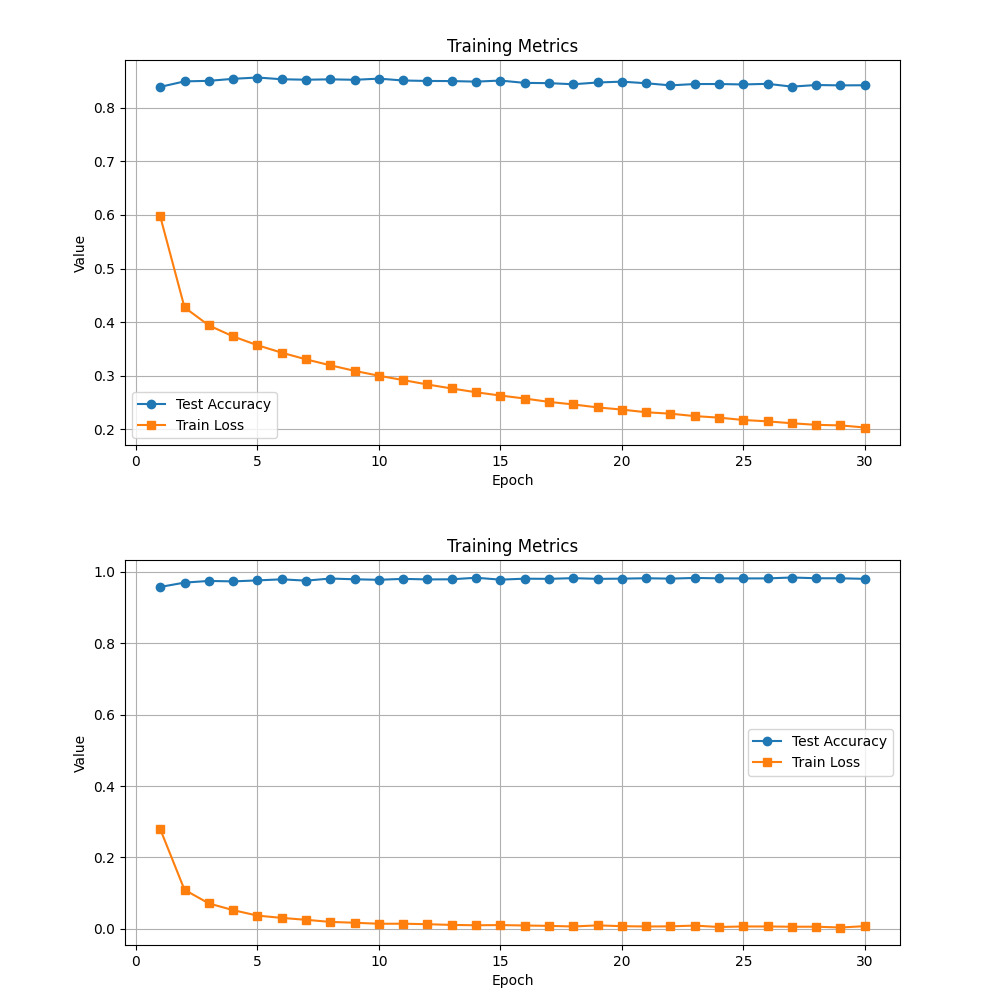
\includegraphics[width=0.8\linewidth]{img/metrics_graph_EMNIST_up.jpg}
    \caption{Metrics graph: the bottom graph shows the MNIST dataset, while the upper graph shows the EMNIST dataset}
    \label{fig:graph_metrics}
\end{figure}

\noindent
As can be seen from \autoref{fig:graph_metrics}, for both networks the accuracy saturates after approximately \(5\) epochs. \\
However, for the MNIST dataset, the test accuracy also saturates after approximately \(10\) epochs, whereas for the EMNIST dataset the test accuracy saturates after approximately \(30\) epochs. \\
The weights and biases matrix used for inference inside the niosII has been generated after \(30\) epochs of training for both datasets.

\vspace{3em}
\noindent
\textit{Note: Even if the accuracy for the EMNIST dataset is approximately \(85\%\), the dataset contains letters that occupy the entire \(28 \times 28\) matrix, while on the LCD writing area (after downscaling) the letters usually occupy a smaller region. \\
For this reason, the training was performed by reducing the size of the dataset letters. \\
This effect can also be seen in \autoref{fig:emnist_char_confrot} where the letter from the dataset is bigger than the one written manually on the screen.}

\subsection{Neural Network inference time}
\label{sssec:nn_inf_time}

Once the neural network had been implemented on the FPGA, two operations were performed to improve the inference time.

\begin{itemize}
    \setlength\itemsep{0pt}
    \setlength\parskip{0pt}
    \item A hardware floating-point operator was instantiated to accelerate, through hardware, the mathematical operations involving weights and biases, \\
    mainly additions and multiplications.
    \item The compiler optimization settings were enabled to optimize the generated code (optimization level 3).
\end{itemize}

\noindent
To evaluate the improvement introduced by each modification to the inference time, the inference execution time was measured via software, and the average inference time was analyzed both with and without these optimizations.

\begin{table}[h!]
    \centering
    \begin{tabular}{l c}
    
        \hline
        Optimization & Inference time \\
        \hline
        No hardware fp. operator, No compiler optimization   & \(6.101 \; s\) \\
        No hardware fp. operator, With compiler optimization & \(3.150 \; s\) \\
        With hardware fp. operator, No compiler optimization & \(2.089 \; s\) \\
        With hardware fp. operator and Compiler optimization & \(0.509 \; s\) \\
        \hline
        
    \end{tabular}
    \caption{Inference Time Dependence on Optimization Methods}
    \label{tab:inf_time_confront}
\end{table}

\newpage
\subsection{Project Demonstration}
\label{sssec:project_demo}

The following images show the user drawing a character on the screen and the neural network recognizing the character drawn, then showing it in the letter box area on the top section of the screen. 

\begin{figure}[h!]
    \centering
    \begin{subfigure}[t]{0.45\textwidth}
        \centering
        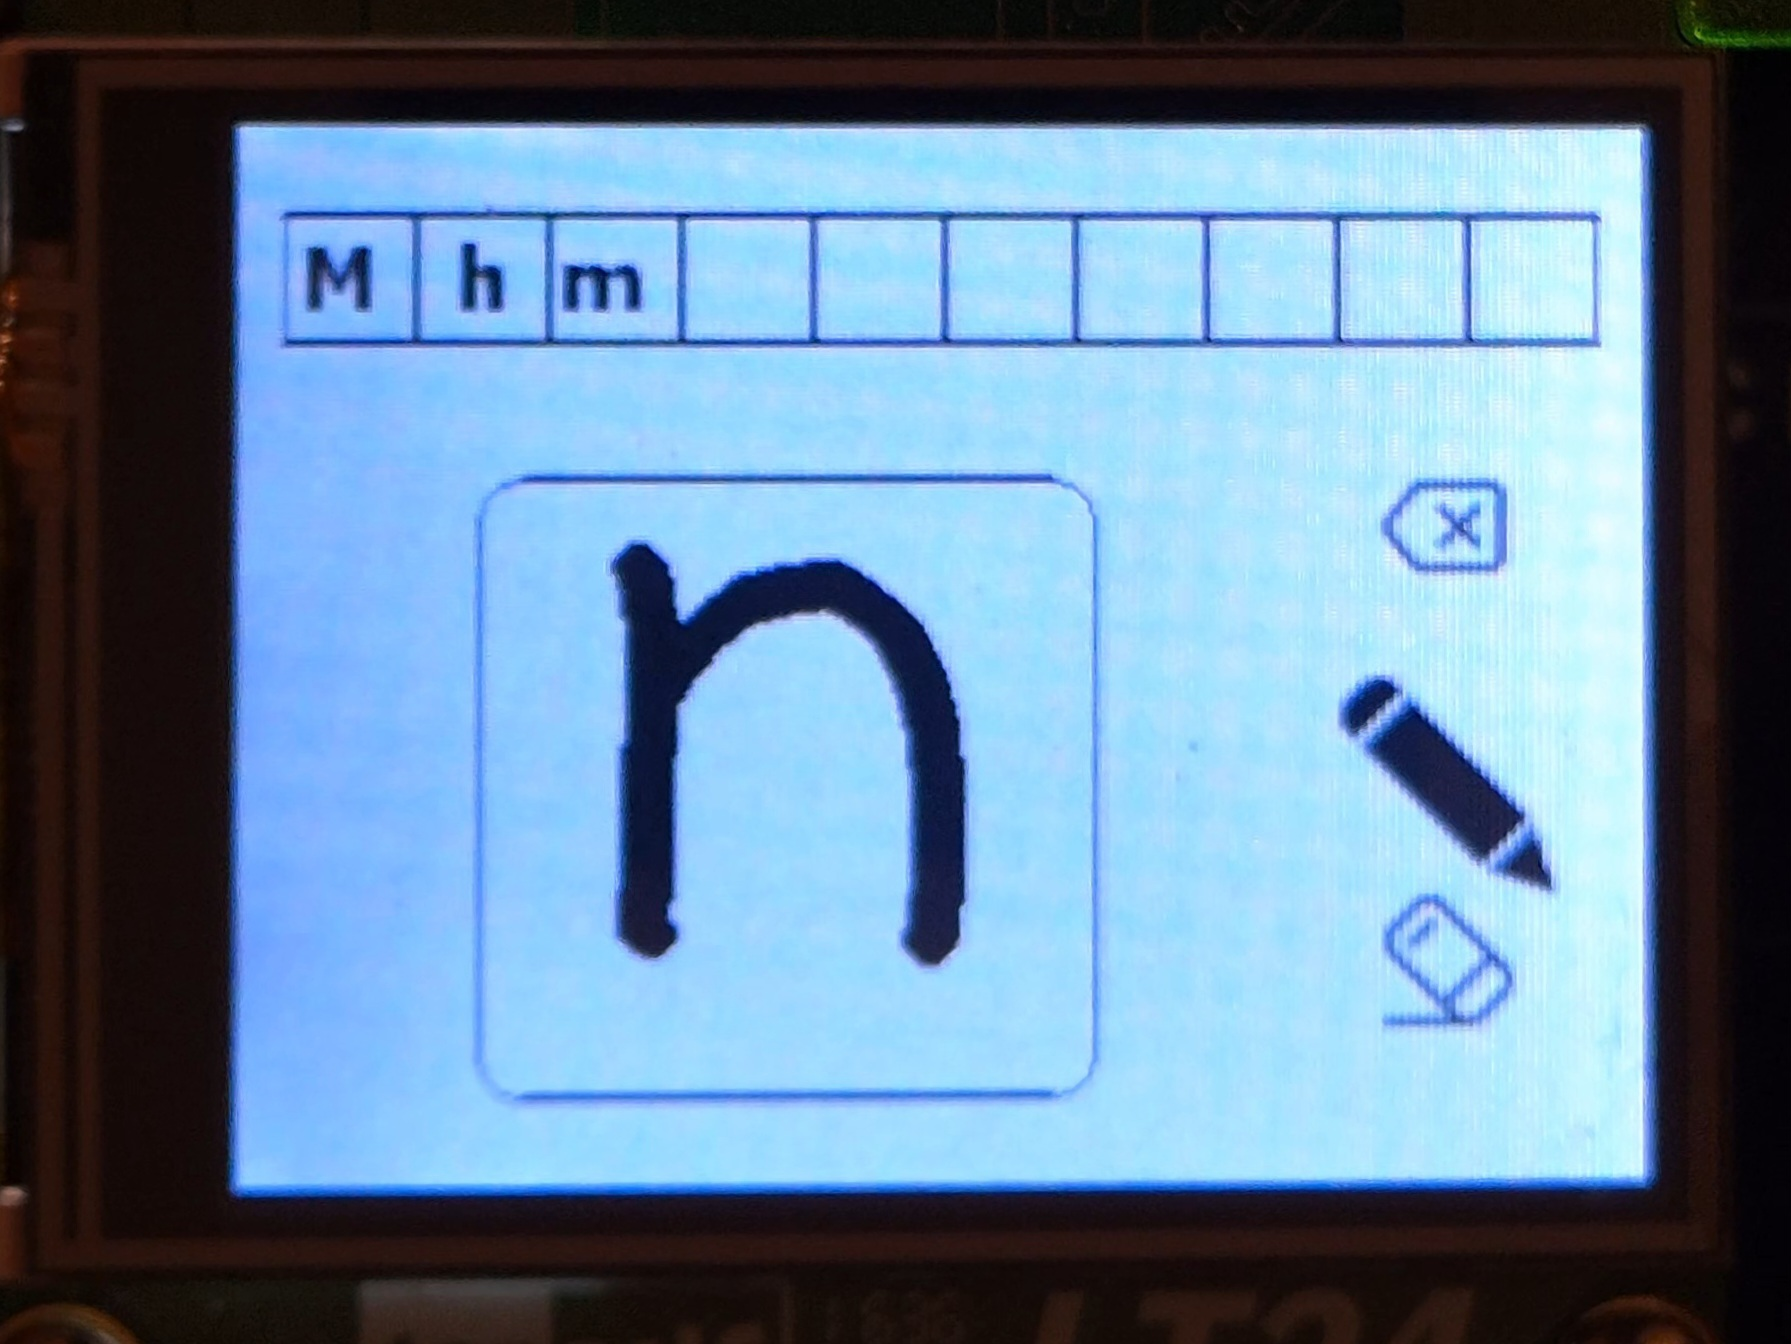
\includegraphics[width=\textwidth, height=3.5cm, keepaspectratio=false]{img/n_drawing.jpg} 
        \caption{Letter "n" drawn by the user}
        \label{fig:sub1}
    \end{subfigure}
    \hfill 
    \begin{subfigure}[t]{0.45\textwidth}
        \centering
        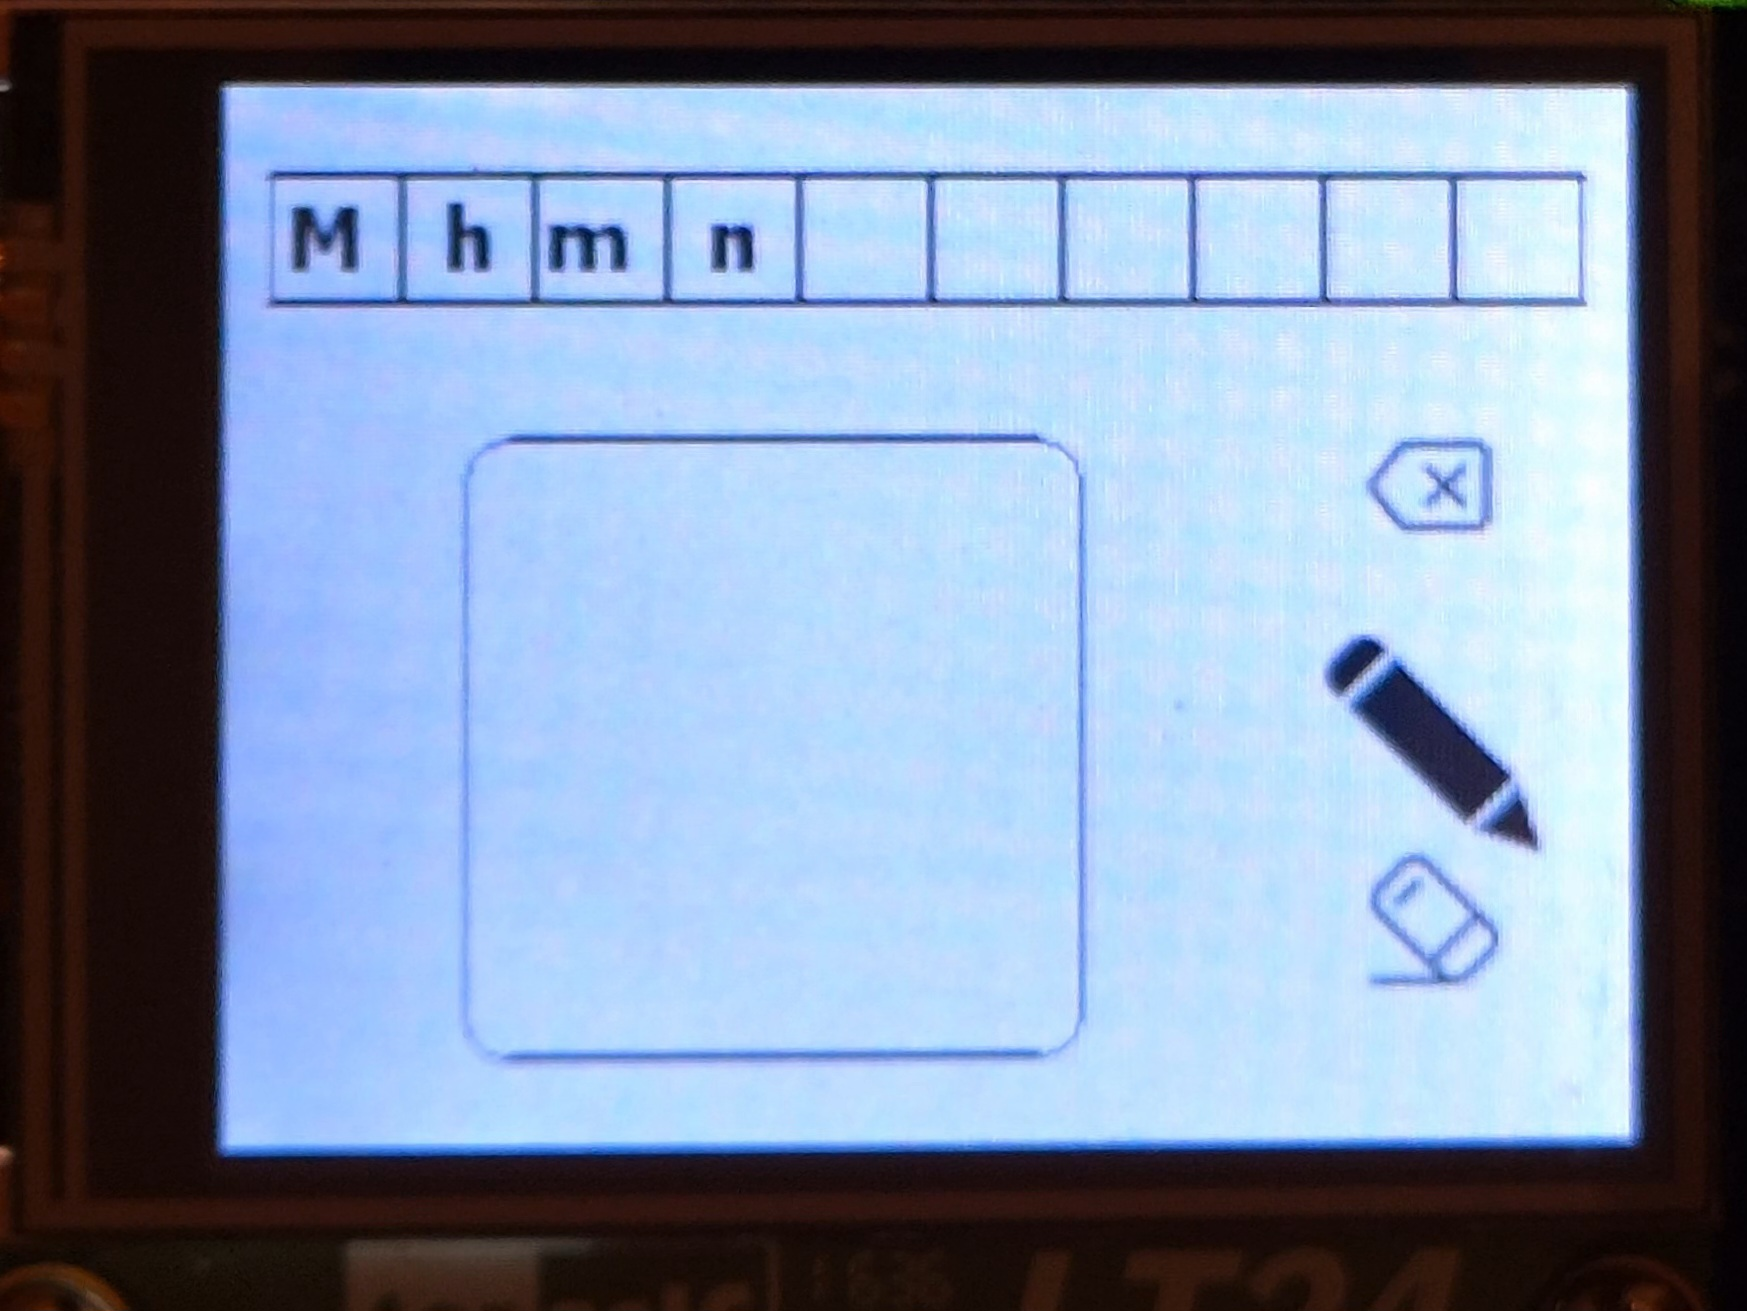
\includegraphics[width=\textwidth, height=3.5cm, keepaspectratio=false]{img/n_letterbox.jpg} 
        \caption{Letter "n" recognized by the NN}
        \label{fig:sub2}
    \end{subfigure}
    
    \caption{Showcasing the recognition of the letter "n"}
    \label{fig:letter_n}
\end{figure}

\begin{figure}[h!]
    \centering
    \begin{subfigure}[t]{0.45\textwidth}
        \centering
        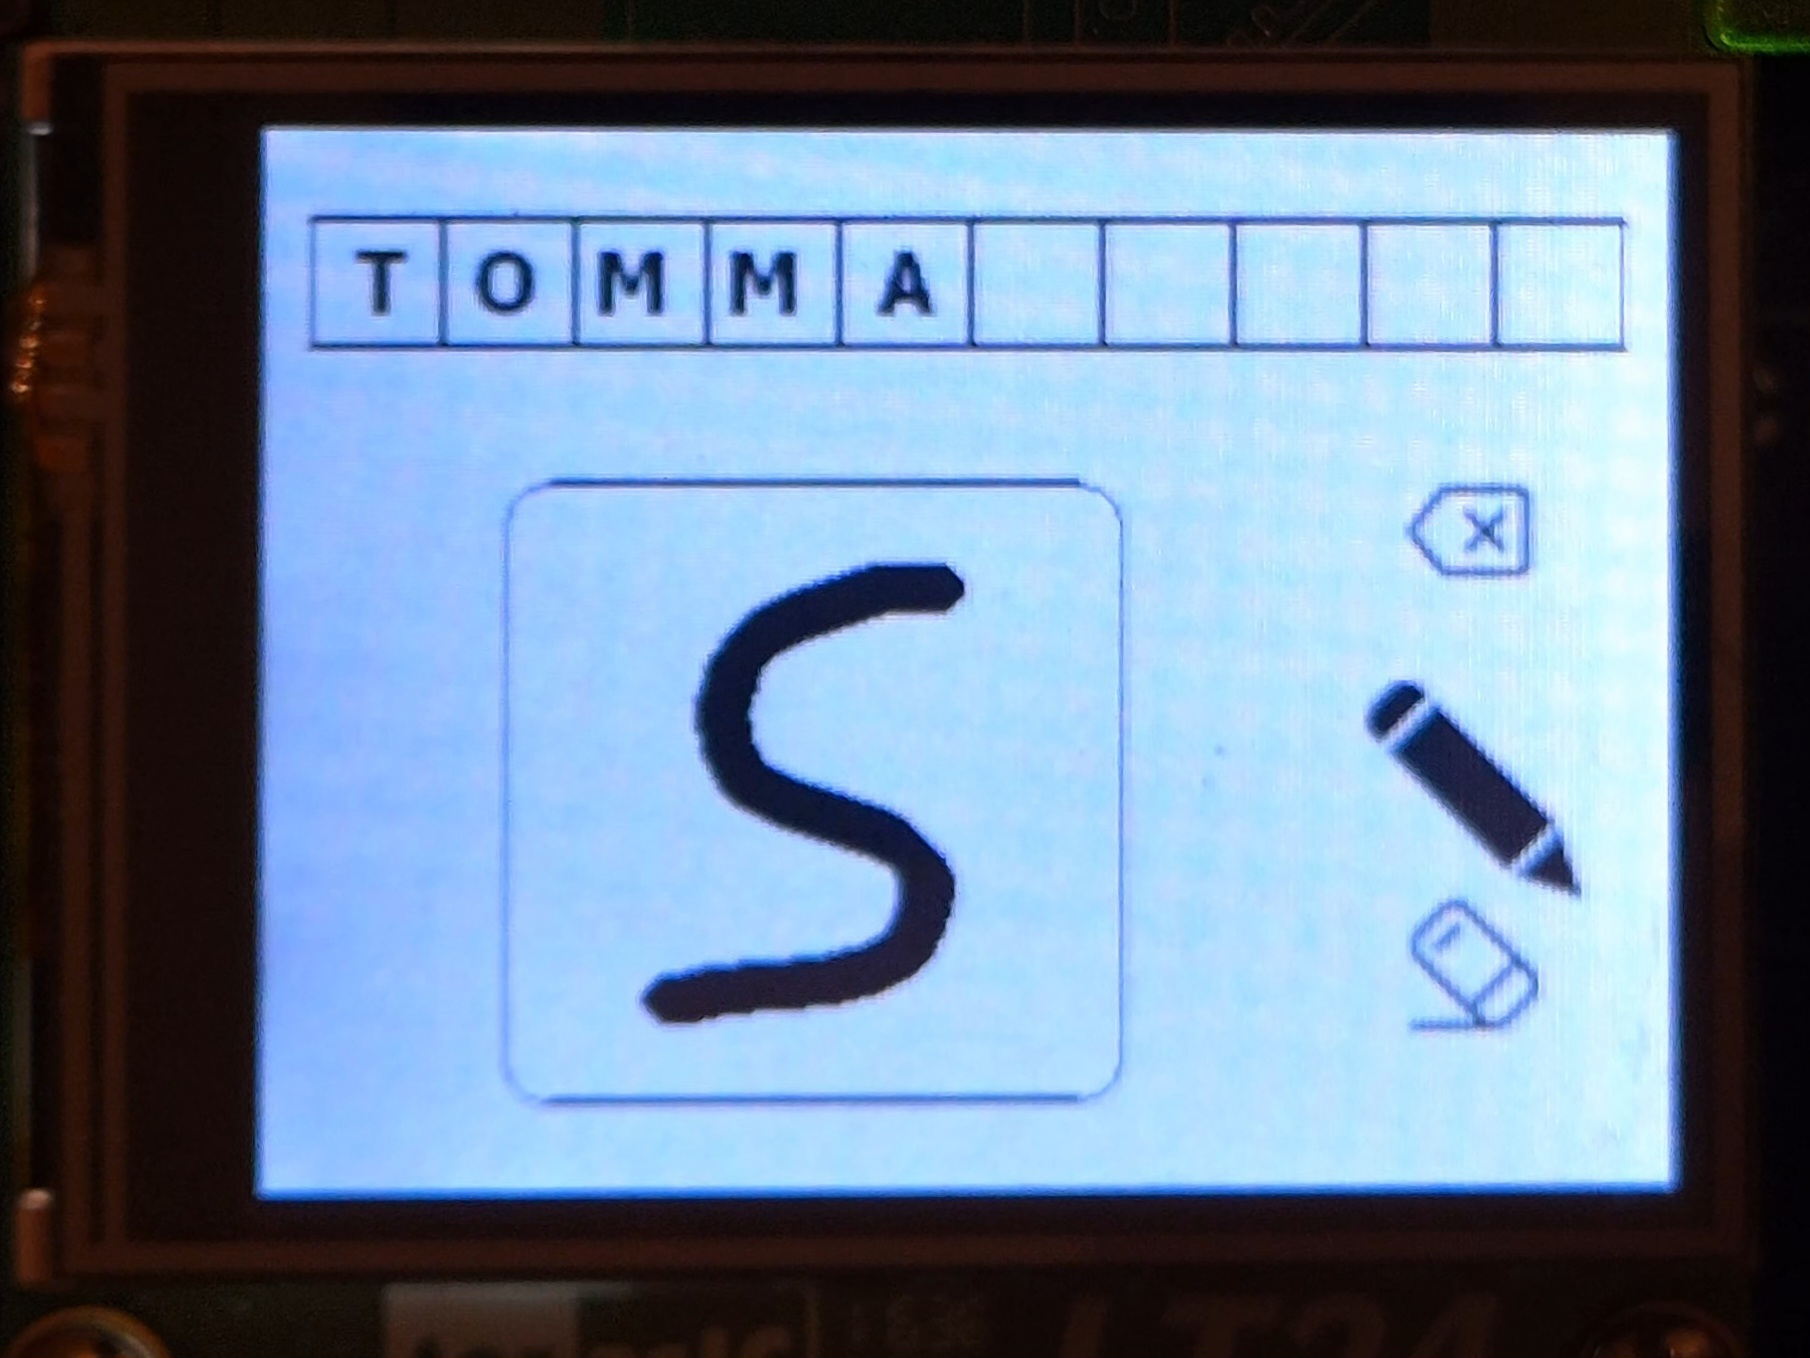
\includegraphics[width=\textwidth, height=3.5cm, keepaspectratio=false]{img/S_drawing.jpg} 
        \caption{Letter "S" drawn by the user}
        \label{fig:sub3}
    \end{subfigure}
    \hfill 
    \begin{subfigure}[t]{0.45\textwidth}
        \centering
        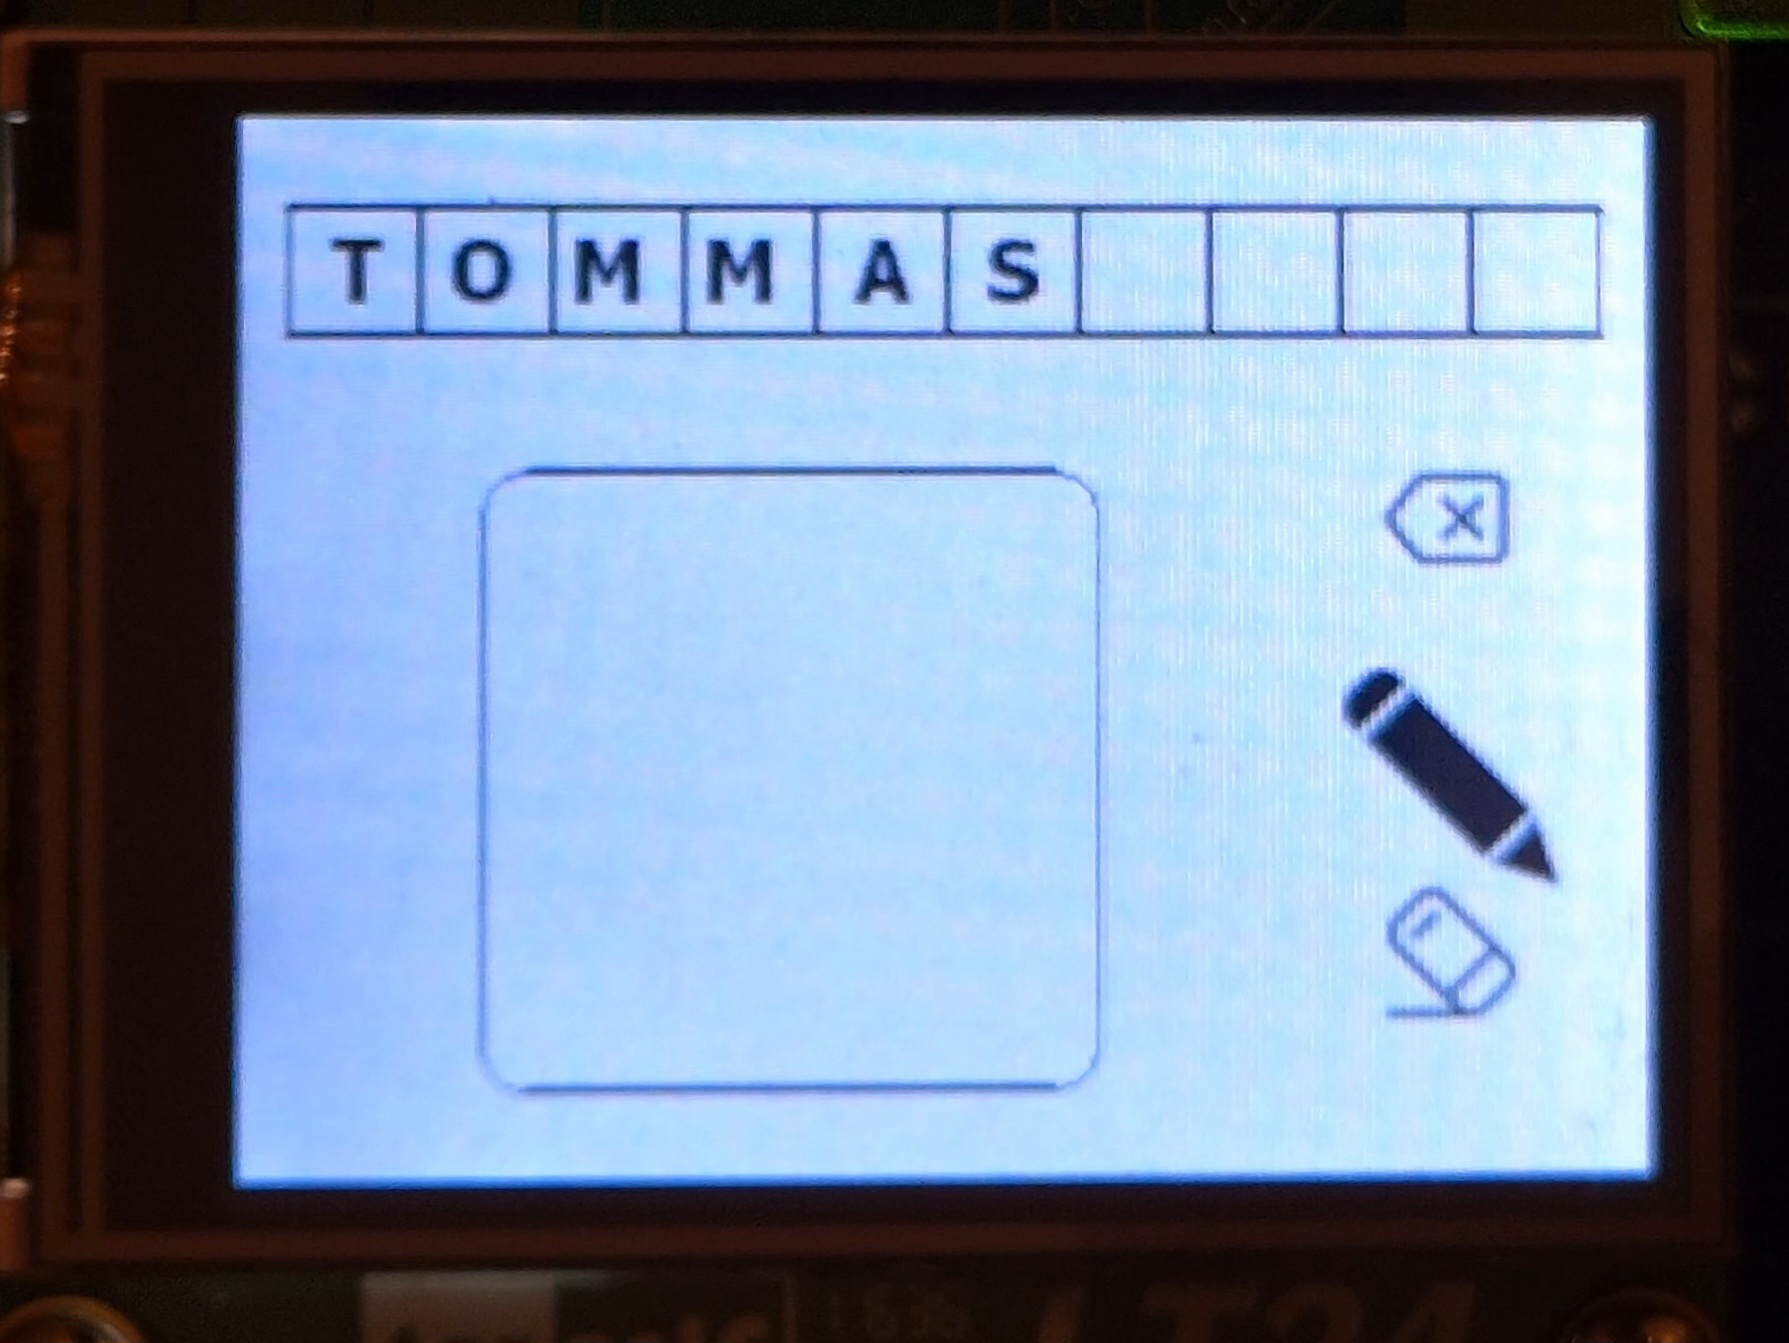
\includegraphics[width=\textwidth, height=3.5cm, keepaspectratio=false]{img/S_letterbox.jpg} 
        \caption{Letter "S" recognized by the NN}
        \label{fig:sub4}
    \end{subfigure}
    
    \caption{Showcasing the recognition of the letter "S"}
    \label{fig:letter_S}
\end{figure}

\begin{figure}[h!]
    \centering
    \begin{subfigure}[t]{0.45\textwidth}
        \centering
        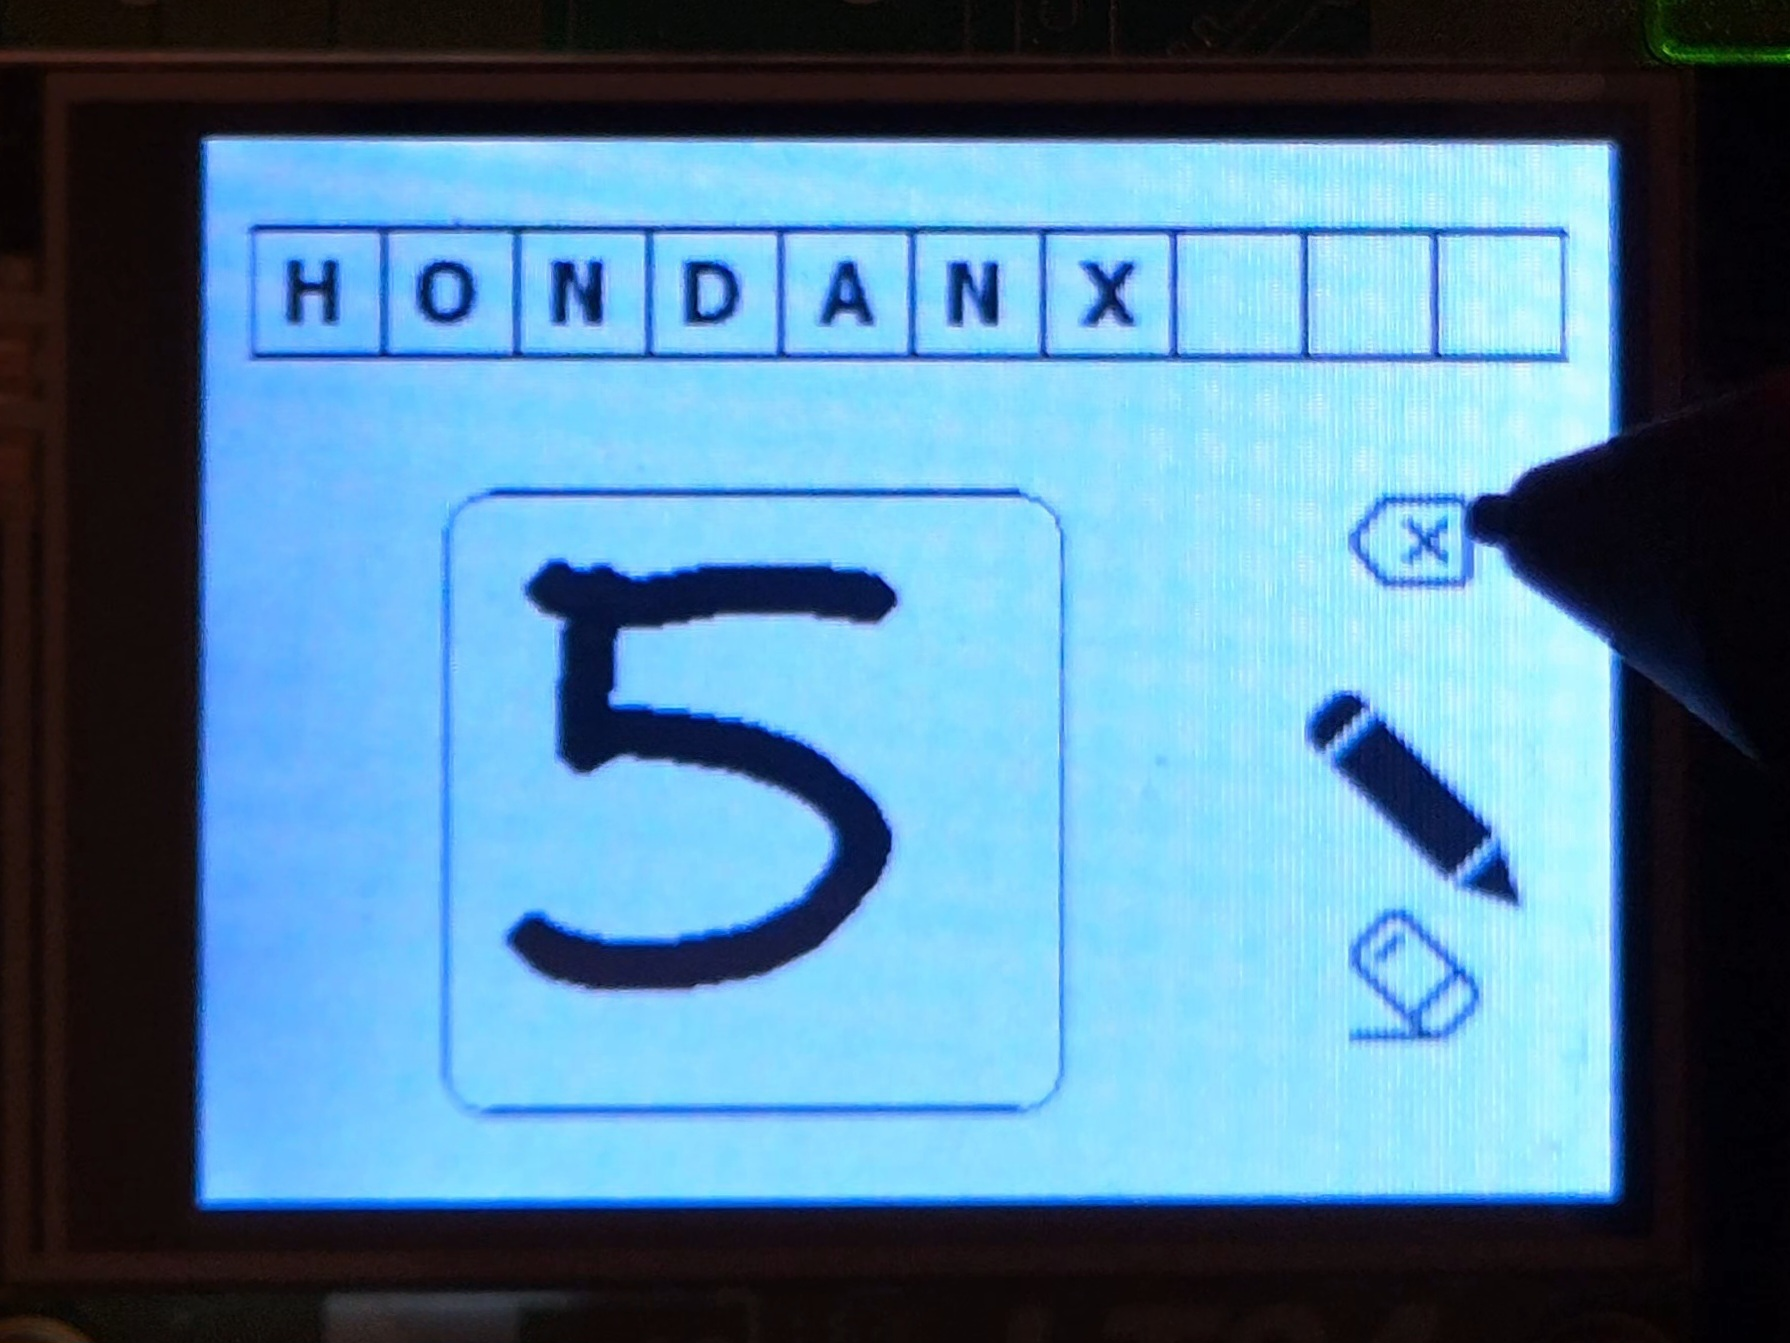
\includegraphics[width=\textwidth, height=3.5cm, keepaspectratio=false]{img/5_drawing.jpg} 
        \caption{Number "5" drawn by the user}
        \label{fig:sub5}
    \end{subfigure}
    \hfill 
    \begin{subfigure}[t]{0.45\textwidth}
        \centering
        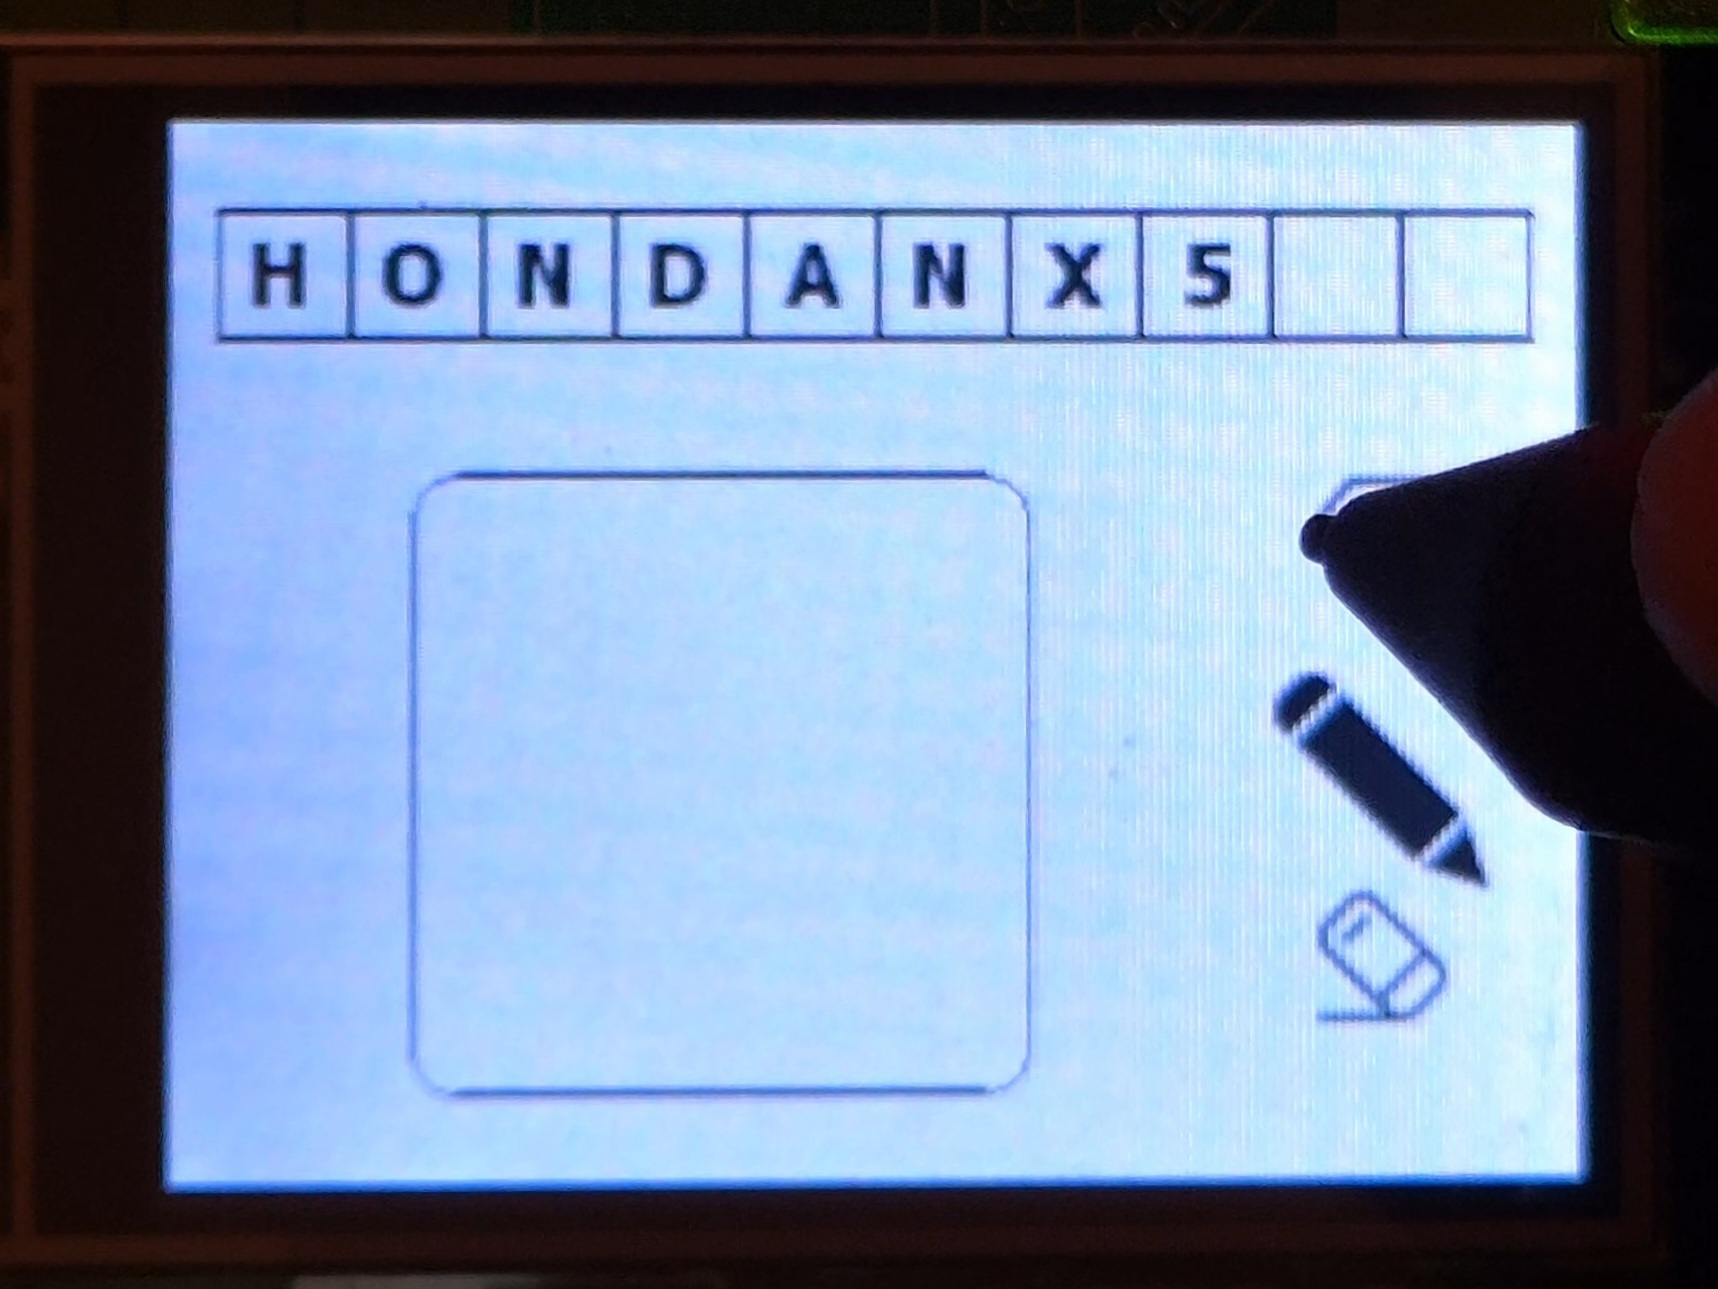
\includegraphics[width=\textwidth, height=3.5cm, keepaspectratio=false]{img/5_letterbox.jpg} 
        \caption{Number "5" recognized by the NN}
        \label{fig:sub6}
    \end{subfigure}
    
    \caption{Showcasing the recognition of the number "5"}
    \label{fig:number_5}
\end{figure}

\newpage
    
    \newpage
    \section{Conclusions}
    The goal of this project was not to achieve a specific level of accuracy with the neural network implemented on the FPGA, but rather to successfully implement the network and obtain an inference time low enough to be unnoticeable to a human user. \\
This requirement was achieved using a complete software implementation while accelerating the floating-point arithmetic operations through dedicated hardware. \\
If this implementation had not been sufficient to achieve an adequately low inference time, several improvements could have been introduced.

\subsection{Possible upgrades}

The possible upgrades are various, but the most important metrics to improve are:

\begin{itemize}
    \setlength\itemsep{0pt}
    \setlength\parskip{0pt}
    \item \textbf{Inference Time}: reducing the inference time is important to compute the output faster.
    \item \textbf{Average Accuracy}: improving the accuracy of the network allows more characters to be recognized correctly on average.
\end{itemize}

\paragraph{Inference time}

In \autoref{sssec:nn_inf_time}, some optimizations and their impact on the inference time of the network are presented. \\
However, if even with these improvements the inference time is not sufficiently small, an alternative approach would be to describe the entire network in hardware using an HDL language and integrate it as a custom module of the CPU. \\
This method is more complex and less modular than a software-based approach, but it can achieve significantly higher speed. \\
If even this solution is not sufficient to meet the inference time requirements, dedicated external hardware accelerators should be used to improve multiply-and-accumulate operations (like GPUs). \\
Another possible approach is to quantize the weights and biases into integer values, simplifying multiplication and addition operations; however, this may lead to reduced accuracy.

\paragraph{Average Accuracy}

The network average accuracy with MNIST dataset, is approximately the \(85\%\), but this value is computed by using some letters from the dataset; the letters wrote on the screen are usually different in orientation and dimensions with the one on the dataset, so the resulting accuracy is less than the one computed (the \(85\%\) accuracy computed during training, see \autoref{sssec:nn_accuracy_tst}). \\
To increase the real accuracy some precaution has been taken, like the one described in the \textit{Note} at the end of \autoref{sssec:nn_accuracy_tst}, but the accuracy remains always lower than \(85\%\). \\
During the test has been tried different types of neural networks, with more hidden layers, or with less hidden layers but with more neurons, but the accuracy increased to the utmost at \(86\%\), the one used for the project is the best compromise of memory-footprint and accuracy of the network. \\
To rise the accuracy a different type of network must be used, like convolutional networks or combination of convolutional and fully-connected networks like LeNet-5 (Reference \cite{lecun1998}). \\
Another limitation is that the network performs poorly when recognizing distorted or scaled letters and numbers. \\
To reduce this problem, the network could be trained using an enlarged dataset generated by applying transformations such as distortion, scaling, and rotation to the original characters.

\vspace{3em}
\noindent
\textit{Note: To compute the real accuracy of the network, different letters would need to be written manually and compared with the expected results. \\
This process can be performed, but it is time-consuming and was not carried out in this project.}

\subsection{Implementation on Different FPGA Devices}

As can be observed in \autoref{sssec:hw_footprint_chpl}, the accelerated floating-point arithmetic project instantiates a significant amount of hardware resources. In particular, the most heavily utilized resources are the embedded 9-bit multipliers: the design instantiates \(16\) of them. \\
Another largely utilized resource is the on-chip memory, with a total usage of \(180,992\) memory bits. \\
These resources are commonly available on most modern FPGAs.

\begin{itemize}
    \setlength\itemsep{0pt}
    \setlength\parskip{0pt}
    \item The MAX10 FPGA (the one we used for this project) has \(288\) available embedded 9bit-multiplier, so their usage for this project is approximately the \(5.5\%\), and \(1,677,312\) memory bits, corresponding to a usage of approximately the \(10.8\%\)
    \item The CycloneII, an Altera older FPGA, has \(70\) available embedded 9bit-multiplier,  so their usage for this project is approximately the \(22.8\%\), and \(483,840\) memory bits, corresponding to a usage of approximately the \(37.4\%\)
\end{itemize}

\noindent
The relatively low resource utilization allows the proposed architecture to be implemented even on older FPGA devices. \\
However, timing analysis may still report violations at the target operating frequency due to technological differences and the lower performance of older FPGA architectures. \\
This results in a lower maximum operating frequency and, consequently, a longer inference time. \\
In some cases, especially in the presence of hold-time violations, the architecture may fail to operate correctly even when the clock frequency is reduced.


    \newpage
    \begin{thebibliography}{}

    \bibitem{lecun1998}
    Yann LeCun, Léon Bottou, Yoshua Bengio, Patrick Haffner (1998) 
    \emph{Gradient-based learning applied to document recognition}, 
    Proceedings of the IEEE, vol. 86, no. 11, pp. 2278--2324. 
    DOI: \href{https://doi.org/10.1109/5.726791}{10.1109/5.726791}.

    \bibitem{rocketboards2024}
    RocketBoards.org (2024) 
    \emph{24" Touch LCD Painter Demo on Atlas-SoC}. 
    Available at: \href{https://www.rocketboards.org/foswiki/Projects/24TouchLCDPainterDemoOnAtlasSOC}
    {rocketboards.org} 

    \bibitem{terasic_lcd}
    Terasic (2015) 
    \emph{LT24 2.4-inch Touch LCD Module / Atlas-SoC Kit Resources}. 
    Available at: \href{https://www.terasic.com.tw/cgi-bin/page/archive.pl?Language=English&CategoryNo=65&No=892&PartNo=2}
    {terasic.com.tw} 

    \bibitem{terasic_de10lite}
    Terasic (2015) 
    \emph{DE10-Lite Development and Education Board}. 
    Available at: \href{https://www.terasic.com.tw/cgi-bin/page/archive.pl?Language=English&CategoryNo=234&No=1021}
    {terasic.com.tw}

    \bibitem{pytorch_nn}
    PyTorch (2024) 
    \emph{Defining a Neural Network}. 
    Available at: \href{https://docs.pytorch.org/tutorials/recipes/recipes/defining_a_neural_network.html}
    {pytorch.org} 

    \bibitem{deeplearningmath_fcnn}
    Liquet, B., Moka, S. and Nazarathy, Y. (2021) 
    \emph{General Fully Connected Neural Networks}. 
    Available at: \href{https://deeplearningmath.org/general-fully-connected-neural-networks}
    {deeplearningmath.org}

    \bibitem{altera_jtag_constraints_2026}
    Intel Corporation (2026) 
    \emph{USB Blaster III FPGA Development Cable User Guide: Creating JTAG Timing Constraints in Quartus Prime Software}, 
    Altera Documentation, Section 5.4.1. 
    Available at: \href{https://docs.altera.com/r/docs/864466/current/usb-blaster-iii-fpga-development-cable-user-guide/creating-jtag-timing-constraints-in-quartus-prime-software}{altera.com}.

\end{thebibliography}
		
\end{document}